% Basic setup. Most papers should leave these options alone.
\documentclass{aa}  

\usepackage{textcomp}
\usepackage{graphicx}
\usepackage[varg]{txfonts}
\usepackage{mathtools}

\usepackage{subcaption}
\usepackage{caption}
\captionsetup[table]{labelfont=bf, labelsep=period}
\captionsetup[figure]{labelfont=bf, labelsep=period}
\usepackage{siunitx}
\sisetup{
  separate-uncertainty = true,
  table-number-alignment = center
}
\usepackage{hyperref}% necessary for continued figures, example in section 3
                                % and appendix
\usepackage{lscape}             % to rotate a single page table, example in appendix.
                                % For landscape tables, see the longtable examples.
\usepackage{placeins} 
\usepackage{xcolor}

\usepackage{graphicx}	% Including figure files
\usepackage{amsmath}	% Advanced maths commands

\usepackage{natbib}
\bibpunct{(}{)}{;}{a}{}{,} % to follow the A&A style


\begin{document}

% Title of the paper, and the short title which is used in the headers.
% Keep the title short and informative.
    \title{Novel insights on the Coma Cluster kinematics with DESI. I. Linking mass profile, orbital anisotropy and galaxy populations}

    \titlerunning{The Coma Cluster kinematics with DESI}

% The list of authors, and the short list which is used in the headers.
% If you need two or more lines of authors, add an extra line using \newauthor
    \author{
        S. Pedratti\inst{1}\thanks{E-mail: s.pedratti1@campus.unimib.it},
        L. Pizzuti\inst{1,2},
        M. Fossati\inst{1,3},
        A. Biviano\inst{2,4},
        A. Boselli\inst{5},
        A. Ragagnin\inst{2},
        A. Carlin\inst{1}
        }
% List of institutions
    \institute{Dipartimento di Fisica G. Occhialini, Universit\`a di Milano-Bicocca, Piazza della Scienza 3, 20126 Milano, Italy
	\and    
        INAF -Osservatorio Astronomico di Trieste, via G. Tiepolo 11, I-34143 Trieste, Italy
    \and
        INAF - Osservatorio Astronomico di Brera, via Brera 28, 20121 Milano, Italy
    \and IFPU $-$ Institute for Fundamental Physics of the Universe, via Beirut 2, 34014 Trieste, Italy
    \and 
    Aix Marseille Univ, CNRS, CNES, LAM, Marseille, France\thanks{Scientific associate INAF - Osservatorio Astronomico di Cagliari, Via della Scienza 5, 09047 Selargius (CA), Italy}
}
%$^{1}$\thanks{E-mail: s.pedratti1@campus.unimib.it}

% These dates will be filled out by the publisher
\date{Received XXXX}

% Enter the current year, for the copyright statements etc.

% Don't change these lines
% Abstract of the paper
 %\textcolor{red}{The abstract is too long. You have to rephrase it to be strictly to the point: "In this paper we investigate the kinematical properties of the Coma galaxy cluster using a new, large sample of spectroscopic data of the member galaxies, collected by the Dark Energy Spectroscopic Instrument (DESI). By means of the \textsc{MG-MAMPOSSt} code, which is based on the Jeans' equation, we jointly reconstruct the total cluster mass profile and the velocity anisotropy profile..." poi devi dire: "abbiamo ottenuto questo valore per la massa usando un NFW (e metti SOLO quello di riferimento), e puoi aggiungere "we discuss the impact of the mass parametrisation and compare our results with previous estimates". Poi dici che hai diviso per campione, e che hai confermato che le galassie rosse hanno orbite più isotrope. Lo stato dinamico di Coma è stato assessed con $A^2$ e sottostrutture, e che hai notato una consistente variazione di velocità per le blue galaxies che potrebbe essere compatibile con un eccesso di densità entrante in Coma lungo la linea di vista. Se ti viene più di 15 righe devi tagliare.}
\abstract{We investigate the kinematic properties of the Coma galaxy cluster using a new, large, spectroscopic sample of member galaxies, from the Dark Energy Spectroscopic Instrument (DESI). By means of the \textsc{MG-MAMPOSSt} code, which is based on the Jeans equation, we jointly reconstruct the total cluster mass profile and the velocity anisotropy profile. Assuming a Navarro-Frenk-White model, we estimate a virial mass $M_{200} = 1.08_{-0.09}^{+0.08}~({\rm stat}) \pm 0.09~({\rm syst}) \times 10^{15} \, \mathrm{M}_\odot $, corresponding to $r_{200}=2.12 \pm 0.06 \, \mathrm{Mpc}$ and a scale radius for the mass profile $r_{\rm s} =0.48^{+0.27}_{-0.13} \, \mathrm{Mpc}$, which provides the tightest robust kinematic mass profile constraint up-to-date. By considering separately the mass of the hot gas and the galaxy stellar mass, we further determine the dark matter mass profile, with $M_{200}^{\rm DM} = 8.6^{+1.2}_{-0.8}\times 10^{14}\,\text{M}_\odot$. We discuss the impact of the mass and number density parametrisations, the effect induced by different choices of the cluster's rest frame and of the radial range of the kinematic analysis, further comparing our results with previous estimates from the literature. The cluster dynamical state has also been assessed, using the spatial and line-of-sight velocity distributions of the members.

We further perform a kinematic study of different subsamples of galaxy populations, selected based on their colour (red sequence, green valley, and blue cloud), focusing in particular on the anisotropy profiles and line-of-sight velocity distributions. 
The orbits of green valley and blue cloud galaxies appear to be more radial in the centre and in the outskirts, respectively, with the latter predicting a higher cluster virial mass. %This, together with the detection of a significant line-of-sight velocity distortion among blue galaxies outside substructures, is consistent with suggests an excess of infalling galaxies along the line-of-sight towards the Coma cluster. %; we interpret this result as an indication of a  filamentary-like structure along the line-of-sight, as further suggested by the analysis of available cosmological simulations.
%We further detect a significant line-of-sight velocity distortion among blue galaxies outside substructures, which is consistent with an excess of infalling galaxies along the line-of-sight towards the Coma cluster; we interpret this result as an indication of a  filamentary-like structure along the line-of-sight, as further suggested by the analysis of available cosmological simulations.

This study provides new insights on the interplay between dynamical and intrinsic properties of galaxies in massive structures, fundamental to verify the tight connection between galaxy evolution and their environment.}
%This study provides a robust foundation for future analyses of the interplay between dynamical and morphological properties of galaxies in clusters, essential to unveiling their diversity and connection with the global cluster environment.}

%We have first studied the numerical density profile of member galaxies on the plane of the sky, which is well-fitted by a projected Navarro-Frenk-White model with a scale radius $r_\nu = 0.71^{+0.07}_{-0.06} \, \mathrm{Mpc}$. We also examined the line-of-sight velocity distributions of the different subsamples, evaluating deviations from Gaussianity, finding indications of near virialization for red sequence galaxies and evidence of ongoing infall stages for blue cloud and green valley galaxies. 

%We have then analysed the full sample of member galaxies with \textsc{MG-MAMPOSSt}, which solves the Jeans' equation in the projected phase space of galaxies $(R,v_z)$, where $R$ is the projected distance from the centre and $v_z$ the velocity measured along the line-of-sight in the cluster's rest frame. The robustness of the mass and anisotropy profile reconstruction has been assessed by adopting different parametric models, i.e. NFW, Burkert and Hernquist for the mass and Tiret and Osipkov-Merritt for the anisotropy, identifying the ones best fitting the observed data using the BIC criterion. In this way we selected the Navarro-Frenk-White and Osipkov-Merritt as the preferred models, with the relative estimate for the Coma Cluster virial mass $M_{200} = 1.03_{-0.08}^{+0.10} \times 10^{15} \, M_\odot $, corresponding to $r_{200}=2.07_{-0.06}^{+0.07} \, \mathrm{Mpc}$ and a scale radius for the mass profile $r_{\rm s} = 0.53_{-0.22}^{+0.11} \, \mathrm{Mpc}$. The anisotropy profile indicates the presence of predominantly radial orbits in the outer regions of the system and orbits closer to isotropy in the innermost part, suggesting a dynamical transition with radius. A clear difference in the central anisotropy emerges when red sequence, green valley and blue cloud galaxies are considered separately, with the RS exhibiting a similar behaviour to the full sample, while GV and especially BC galaxies move preferentially along radial trajectories; these results are consistent with the general scenario of morphological evolution driven by the higher efficiency of ram-pressure stripping on elongated orbits.

%We then apply the DS+ code to identify group-sized substructures in the Coma Cluster, using a method that only requires the projected positions and line-of-sight velocities of member galaxies. We find 7 different substructures, with the two largest ones (SW and NW of the centre) that are consistent with the results of previous notable studies of Coma Cluster substructures. The deviation of the LoS velocity distribution from a Gaussian profile is not resolved by removing galaxies associated with substructures. This suggests the presence of a filamentary structure, from which galaxies located within the projected virial region are infalling toward the cluster centre.


% Select between one and six entries from the list of approved keywords.
% Don't make up new ones.

\keywords{Galaxy: evolution -- galaxies: clusters: individual: Coma -- galaxies: kinematics and dynamics}

\maketitle
%%%%%%%%%%%%%%%%%%%%%%%%%%%%%%%%%%%%%%%%%%%%%%%%%%

%%%%%%%%%%%%%%%%% BODY OF PAPER %%%%%%%%%%%%%%%%%%

\section{Introduction}
\label{sec:intro}

Galaxy clusters, the largest gravitationally-bound systems in the Universe, are excellent laboratories at the crossroads of cosmology and astrophysics. 
In order to employ clusters as reliable cosmological probes, it is essential to use robust methods to estimate their total mass, as well as the radial mass distribution. These can provide fundamental insights on the dark matter properties \citep[\textit{e.g.}][]{Biviano:2023oyf,Vall_s_P_rez_2025} and the nature of gravity \citep[\textit{e.g.}][]{Pizzuti22,Zamani24}.
%and the evolution of galaxies in dense environments (\textit{e.g.} \citealt{Sampaio_2024}). 

In parallel, the deep potential wells of galaxy clusters make them % behave almost as closed systems, retaining most of their gas and galaxies, making them 
particularly convenient to study the processes affecting galaxy evolution and feedback scenarios in dense environments (\textit{e.g.} \citealt{Boselli_2014,Boselli_2022,Sampaio_2024}). In particular, galaxy populations in clusters are predominantly composed of massive, red, quiescent galaxies with low star formation rates, generally referred to as 'Early-Type' galaxies (ETGs), alongside a smaller population of low-mass, blue, highly star-forming galaxies, known as 'Late-Type' galaxies (LTGs) \citep{Dressler_1997, Boselli_2006}.  %Is this variety of populations due to 'Nature or Nurture'? In other words, are the galaxies' features determined only by the initial conditions of their formation or are they determined and shaped by interactions with the environment in which they evolve? 

The features of galaxies in clusters are determined by a combination of the initial conditions of their formation and the interactions within the environment in which they evolve. How these two aspects impact the observed population of galaxies in clusters is hotly debated in the astrophysics community. Ram-pressure stripping of the interstellar medium (ISM) is considered as the dominant mechanism to affect the properties of galaxies in clusters \citep{Boselli_2022, Xie_2025}: as they travel at high velocities (up to $\sim 1000$ km/s) through the hot and dense gas of the Intra-Cluster Medium, the ISM can be stripped away if ram-pressure overcomes the gravitational pressure anchoring the gas to the galaxy \citep{Gunn_1972}.
This process is more effective for galaxies on radial orbits, which both increase their speed and bring them closer to the cluster core \citep{Vollmer_2001, Singh_2019}. 

Moreover, \citet{Tammann72}, \citet{MD77}, \citet{Sodre+89}, \citet{Biviano+92}, \citet{Colless_1996}, \citet{ABM98}, and later \citet{Boselli_2006}, showed that the line-of-sight (LoS hereafter) velocity distributions of galaxies in clusters is type-dependent. While ETGs display a virialised Gaussian velocity distribution, LTGs exhibit strong deviations from Gaussianity, being the distribution generally broader and, in some cases, asymmetric \citep{ZF93,Biviano+97}. These differences in velocity distributions are probably due to LTGs orbits being more elongated and to their anisotropic infall from the surrounding large scale filaments,
and serve as an indirect evidence for their infall onto the cluster core (\textit{e.g.} \citealt{Mamon_2019,Pizzuti_2025b}). The more elongated orbits of spiral, gas-rich, star forming galaxies in dense environments suggest that these galaxies are subject to dynamic gas depletion, mainly due to ram pressure stripping, leading to star formation quenching and morphological transofrmations of LTGs into ETGs, eventually producing the predominant population of red quiescent systems of present day clusters.
\medskip

%We too have performed the LoS velocity distribution analysis for the Coma Cluster, with our newest sample, and the results can be found in Sect.~\ref{subsec:vel distrib}.

%The overall picture seems to suggest that when a spiral, gas-rich, star forming galaxy is captured by the gravitational potential of a cluster and moves on elongated orbits towards its centre, it undergoes severe gas depletion, mainly due to ram pressure stripping, and star formation is quenched as a consequence. This sets off the transition from a LTG to an ETG, producing the observed predominant population of red quiescent systems in the cores of clusters. 
%Another supporting evidence for this interpretation of the evolution of galaxies in clusters is the so-called 'Butcher-Oemler' effect \citep{Butcher_1978}: at higher redshifts there appears to be a larger fraction of blue galaxies in the clusters cores than are seen in the core of clusters in the Local Universe, suggesting that star formation in these dense environment has been shut down in recent times of cosmic history. 


This paper focuses on the Coma Cluster (Abell 1656), one of the most massive and well-studied galaxy clusters of the Local Universe at a redshift $z = 0.023$ \citep{Kang_2025}, whose study is favoured by its position in the sky near the Milky Way's north pole, where contamination due to dust and gas from our galaxy's plane is negligible. Despite early indications of the presence of subclustering \citep[see][and references therein]{Biviano98}, the Coma cluster has been considered for a long time as the prototype of an old and relaxed cluster. X-ray maps \citep{White_1993, Neumann_2001}, analyses of projected distribution of galaxies \citep{Baier_1990} and LoS velocity distributions \citep{Colless_1996} established the existence of a group centred around the massive galaxy NGC 4839, that is now understood to be on secondary infall after reaching its first orbital apocentre \citep[\textit{e.g.}][]{Biviano+96,Lyskova+19,Churazov_2021}. In addition, a recent or ongoing merger has been identified between the main cluster and a group, partially disrupted, originally dominated by NGC 4889 or NGC 4874 \citep{Biviano+96,Adami_2005a}. Much more recently, \citet{Costa_2025} and \citet{Kang_2025} found evidence of many substructures, often overlooked because of the faint nature of the galaxies tracing them. The interactions that result from this complex configuration could be at the origin of the observed post-starburst (PSB) galaxies in the periphery of the cluster \citep{Caldwell_1993, Gavazzi_2010}. 

\medskip
%Note that beside the Jeans analysis, alternative kinematic approaches such as the caustic method \citep{Diaferio99,Jimenez_2025}, machine-learning mass estimators \citep[see, e.g.,][]{Ntampaka+15,Ho_2022} and other non-parametric frameworks are commonly used. Independent constraints are also provided by X-ray hydrostatic analyses \citep[see, e.g.,][]{Ettori_2013} and gravitational lensing measurements \citep[see, e.g.,][]{Umetsu_2020}. 
After \citet{Zwicky33}'s first estimate of the total mass, many studies focused on getting more precise determinations of the total mass distribution through several independent measurements. More specifically, \citet{Lokas_2003} performed a kinematic analysis of elliptical galaxies in the cluster field to obtain a total mass $M_{200} = 1.2 \times 10^{15} \, M_\odot$\footnote{All quantities presented in this paper are referred to a cosmological model with $H_0=70$ km~s$^{-1}$~Mpc$^{-1}$, $\Omega_m=0.3$, and $\Omega_{\Lambda}=0.7$.} with $30\%$ accuracy, within a corresponding radius $r_{200}=2.2 \, \mathrm{Mpc}$ . Here and throughout the paper, we refer to  $M_\Delta = \Delta \,H^2(z)/(2G)\times r_{\Delta}^3$ as the cumulative mass enclosed in a radius $r_{\Delta}$ of a spherical overdensity with an average density $\Delta$ times the critical density of the Universe at the cluster redshift $\rho_{c}(z)$. Following similar prescription in the literature, we define quantities at $\Delta = 200$ as 'virial' mass and radius, respectively. %The typical mass quantity used in the literature is the virial mass $M_{200}$, i.e. the mass within the virial radius $r_{200}$, defined as the radius within which the average matter density of the system is $200 \rho_{c,0}$, being $\rho_{c,0}$ the critical density of the Universe at $z \sim 0$. Let us now quickly go through some notable virial mass measurements: \citet{Lokas_2003} estimated $M_{100}$ (the analogue of $M_{200}$ with an average density of $100\rho_{c,0}$ instead of $200\rho_{c,0}$) through kinematic analysis of elliptical galaxies, finding a value of $1.4 \times 10^{15} \, M_\odot$ with $30\%$ accuracy, within a radius $r_{100}=2.9 \, \mathrm{Mpc}$. 
Weak lensing calculations allowed \citet{Gavazzi_2009} to estimate $M_{200}=5.1^{+4.3}_{-2.1} \times 10^{14} \, M_\odot$, while a recent paper by \citet{Cha_2025} employed a deep learning approach based on convolutional neural network to mitigate the potential setbacks of traditional lensing analyses, such as noise amplification and mass-sheet degeneracy, finding the value of $M_{200}=7.4^{+2.4}_{-3.1} \times 10^{14} \, M_\odot$. \citet{Mirakhor_2020} combined the electron density profile, recovered from the X-ray observations of \textit{XMM-Newton}, and the pressure profile from the \textit{Planck} Sunyaev--Zeldovich effect~\citep[SZ,][]{Sunyaev1972} observations to estimate the virial mass as $M_{200}=(8.5 \pm 0.55) \times 10^{14} \, M_\odot$, corresponding to a radius $r_{200}=2.0 \, \mathrm{Mpc}$. Finally, \citet{Ho_2022} made use of recently developed methodologies based on Bayesian deep learning, obtaining $M_{200}=1.8^{+0.74}_{-0.53} \times 10^{15} \, M_\odot$ and, even more recently, \citet{Benisty25} employed the caustics, the virial theorem, and the Hubble-flow methods to find virial masses in the range $[1.1-2.9]\, \times 10^{15} \,  M_\odot$.
%$[0.77-2.0]\, \times 10^{15} \,  h^{-1} \, M_\odot$, being $h=\frac{H_0}{100 \, \mathrm{km \, s^{-1} \, Mpc^{-1}}}$. 
%In this work we take as the value of the Hubble parameter today $H_0=H(t=t_0)=70 \, \mathrm{km\,s^{-1} \, Mpc^{-1}}$, in between CMB \citep{Planck_2020} and local distance indicators \citep{Riess_2018} measurements.
 
\medskip
In this work we perform a kinematic analysis of the Coma Cluster's member galaxies, using new spectroscopic data collected from DESI \citep[Dark Energy Spectroscopic Instrument,][]{DESI_DR1} to jointly reconstruct the mass and anisotropy profiles %\citep[\textit{e.g.}][]{Lokas_2003,Mamon_2013}, 
under the assumption that the cluster is in an equilibrium configuration. We employ the \textsc{MG-MAMPOSSt} code of \cite{Pizzuti_2021}, which applies the Jeans equation to the projected positions and LoS velocity distribution of member galaxies. 
We study the relation between the Coma Cluster member galaxies and the global cluster environment, by tracing the behavior of the orbits for different subsamples of galaxies based on their colour (red sequence, green valley, blue cloud), further discussing the impact of systematics due to mass and anisotropy models and different  sample parameters (\textit{e.g.} projected radial ranges, choice of the centre, velocity rest frame).
Our findings provide the stringent constraints on the mass distribution in Coma and on the orbits of its member galaxies to date.
%Our findings reveal an excess of positive LoS velocities for the blue cloud galaxies in the cluster's rest-frame within the projected radius $R \leq r_{200}$; we test the consistency of this results with the presence of an overdensity along the LoS infalling towards the cluster. To this end, we analyse a massive halo at low redshift from a $\Lambda$CDM cosmological hydrodynamic simulation from the DIANOGA-SIDM set of \cite{Ragagnin_2024}.

The work is structured as follows: Sect.~\ref{methods} describes the DESI dataset of galaxies in the Coma Cluster and the preliminary analysis performed on the spatial and velocity distribution of galaxies. In Sect.~\ref{sec:mamposst} we provide an overview of the \textsc{MG-MAMPOSSt} method, employed to study the kinematics of the system, and of the various models adopted in the analysis. In Sect.~\ref{results} we show our results, further discussing the impact of systematic effects and checking the robustness of our analysis. The conclusions and final considerations are reported in Sect.~\ref{sec:conclusions}. 


\section{Dataset and preliminary analyses}
\label{methods}

%This section describes the dataset and methods used for the dynamical analysis of the member galaxies in the Coma Cluster,  performed by employing the \textsc{MG-MAMPOSSt} code \citep{Pizzuti_2021}. This is the first time that this code has been used on the Coma Cluster, which allowed us to perform the very first study of the orbital anisotropy profile of its member galaxies. Before running \textsc{MG-MAMPOSSt}, we perform a first analysis to estimate the numerical density profile of member galaxies and study the distribution of velocities along the LoS for different subsamples, selected based on their colour.

\subsection{Dataset}
\label{subsec:dataset}

Our dataset comes from the first Data Release (DR1) of DESI \citep{DESI_DR1}, a highly multiplexed spectroscopic instrument mounted on the Mayall 4-meter telescope at the Kitt Peak National Observatory. The Coma cluster was targeted by Science Verification (SV) programs, aimed at obtaining a high density of cluster targets. As a result, the final target density in the area is much larger than the average of the DESI survey, providing us with more than 2,000 spectra in a DESI pointing. We removed all the spectra from non-nuclear sources or misclassified stars, through visual and kinematic inspection, respectively, thus obtaining a pure sample of nuclear spectra of galaxies.
We require the objects to have at least $g$- and $r$-band magnitudes ($m_g$ and $m_r$, respectively) for colour selections. We further select only galaxies with $m_r <19.7$ mag to ensure a high spectroscopic completeness of the photometrically selected sample. We estimate the spectroscopic completeness by selecting all the extended (galaxy-like) photometric objects brighter than the magnitude cut, deriving which fraction has available DESI spectroscopy in bins of distance from the centre of the Coma cluster, and excluding the central 100 kpc, as further discussed below. We find an overall spectroscopic completeness of 91\% in our sample, with no significant radial trends.

Our final spectroscopic galaxy catalogue includes 1758 galaxies and covers the angular coordinate range (J2000) $190^\circ < \text{RA} < 200^\circ$ and $25^\circ < \text{DEC} < 31^\circ$, for a total sky area of $\sim 53 \, \deg^2$ around the Coma Cluster region, extending out to $\sim 3\,r_{200}$. We consider the cluster centre to be located at (RA = $194.90 \,\deg$, DEC = $27.96 \,\deg$), corresponding to the  position of the elliptical galaxy NGC 4874 (see \textit{e.g.} \citealt{Malavasi20}). In order to avoid systematics in the kinematic analyses, it is essential to remove the interlopers, i.e. galaxies that are within the virial radius in projection but that are outside the virial sphere. This step has been performed using the Clean algorithm \citep[Appendix B of][]{Mamon_2013}, which provides a more refined approach with respect to a simple phase-space cut. Fig.~\ref{fig:full_distrib_DESI} depicts the projected positions of the 1651 galaxies in our final Coma Cluster sample. 
As we will discuss in Sect.~\ref{sec:mamposst}, our kinematic analysis requires the projected positions $R$ from the cluster centre and the LoS velocities of the member galaxies $v_\text{RF}$, computed in the cluster's rest frame.  The space of pairs ($R,v_\text{RF}$) is called projected phase-space (p.p.s. hereafter), shown in Fig.~\ref{fig:phase_space_DESI}. %The resulting LoS velocity distribution of the member galaxies is further shown in Fig.~\ref{fig:LoS_distrib_DESI}.

\begin{figure}
    \centering
    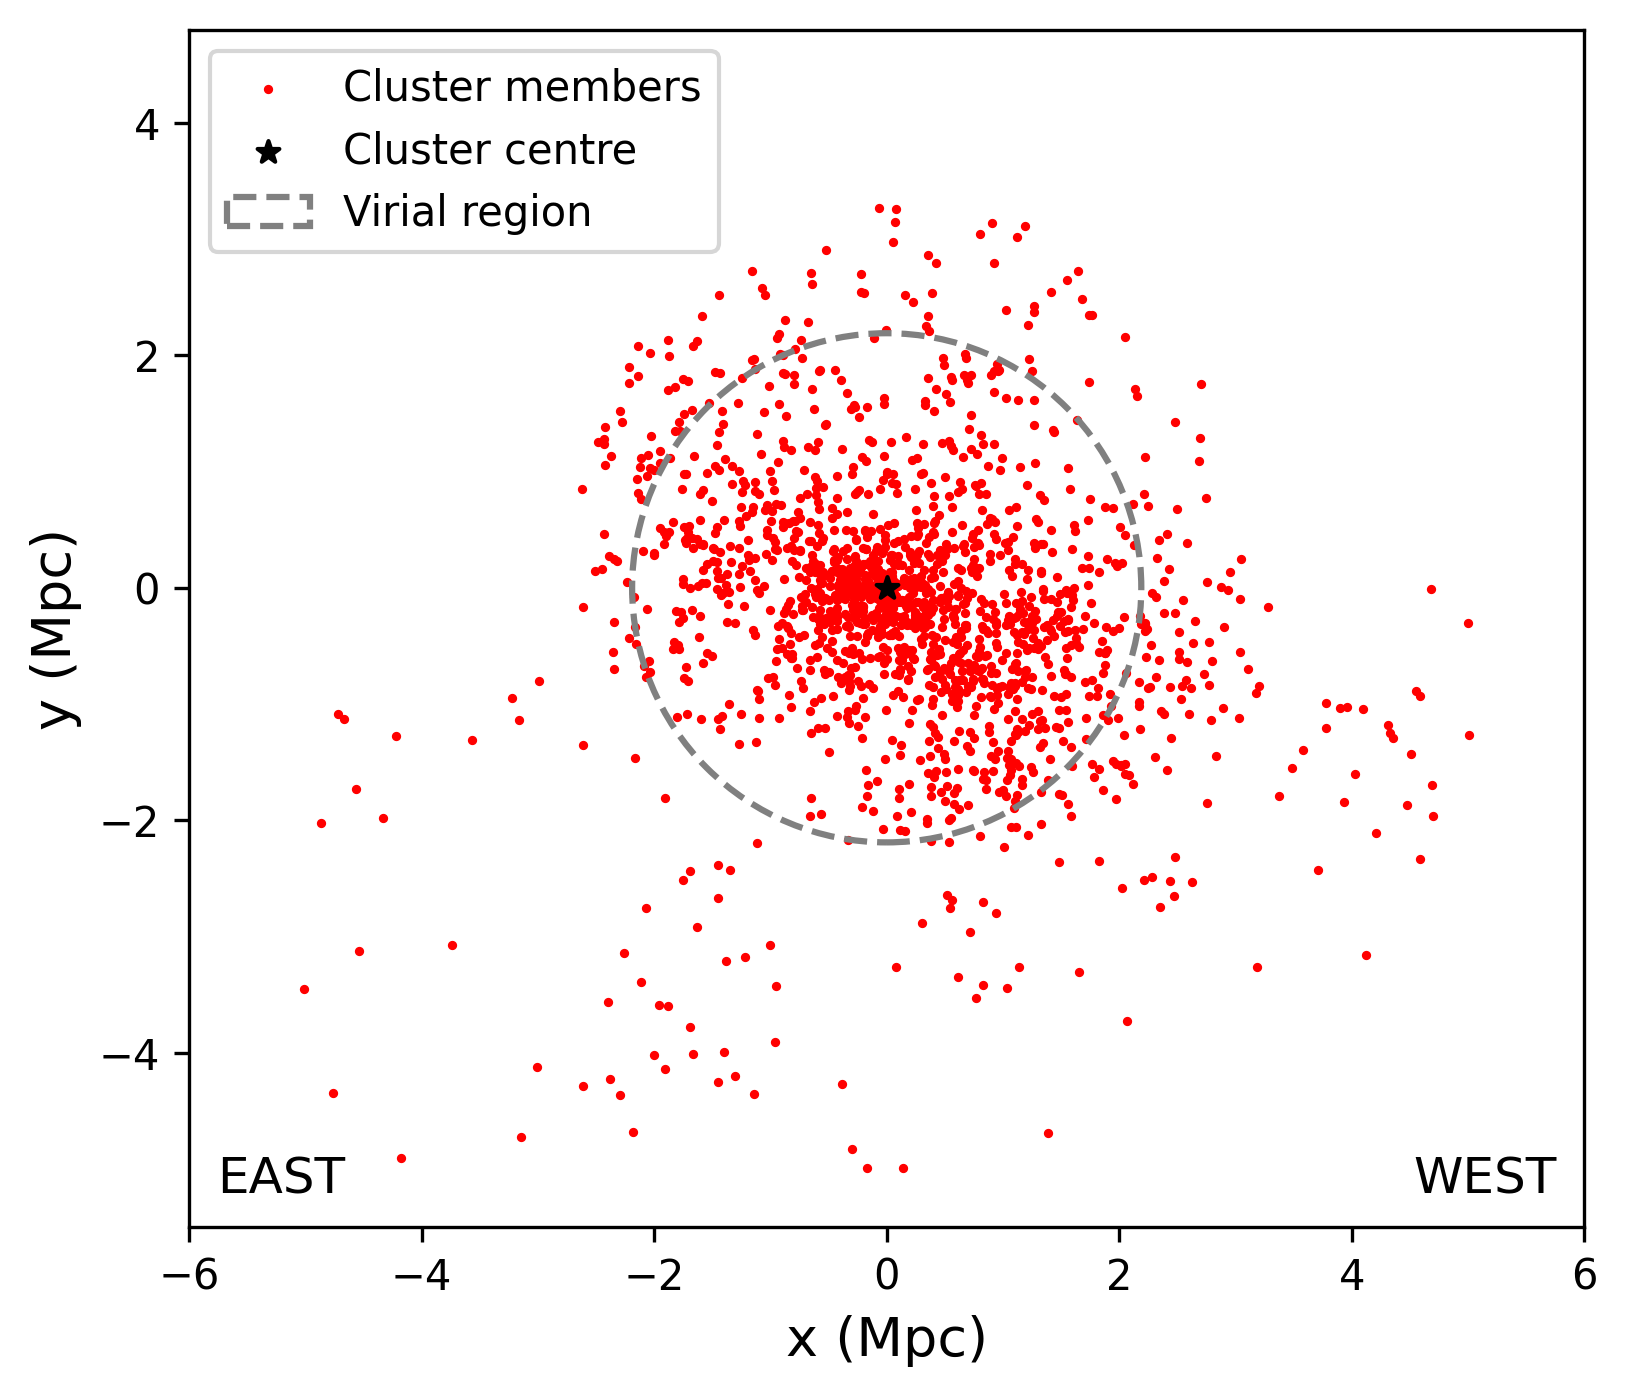
\includegraphics[width=0.85\linewidth]{images/full_pos.png}
    \caption{Projected positions of galaxies in the Coma Cluster. The point marked with a black star indicates the cluster centre, whose coordinates (RA=194.90 deg, DEC=27.96 deg) have been taken from \citet{Malavasi20} as the position of NGC 4874, while the grey circle encloses the region within $r_{200} = 2.19 \, \mathrm{Mpc}$, quoted in \citet{Boselli_2006}. }
    \label{fig:full_distrib_DESI}
\end{figure} 

\begin{figure}
    \centering
    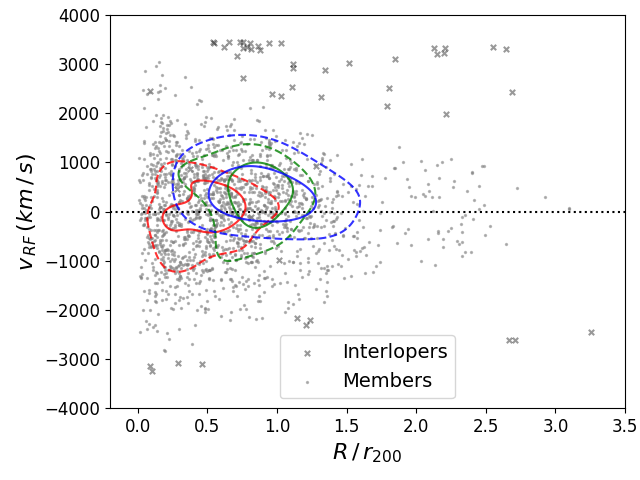
\includegraphics[width=0.9\linewidth]{images/pps_colored.png}
   \caption{Projected phase-space distribution of member galaxies in the Coma Cluster (grey dots) and interlopers removed by Clean (grey crosses). The black dashed line indicates the average velocity of the cluster (Hubble + bulk motion), while coloured curves highlight iso-density contours (dashed and solid lines correspond to 90th and 97th percentiles, respectively) for RS (red), GV (green) and BC (blue) galaxies. The projected distance from the centre is normalized to $r_{200}$, taken equal to the value quoted in \citet{Boselli_2006}, $2.19 \, \mathrm{Mpc}$ }
    \label{fig:phase_space_DESI}
\end{figure}

%\begin{figure}
%    \centering
%    \includegraphics[width=0.9\linewidth]{images/vel_distrib_members.png}
%   \caption{LoS velocity distributions of the full sample of member galaxies. The vertical dashed line indicates the average velocity of the cluster. }
%    \label{fig:LoS_distrib_DESI}
%\end{figure}

In order to study the orbital properties of different galaxy populations, we split the sample into three main categories according to their position in the $(m_g-m_r)$ vs stellar mass ($M_*$) diagram. The stellar masses have been computed from the DESI photometry using CIGALE \citep{Boquien2019} SPS modelling with exponentially declining SFHs, BC03 models and a \cite{Chabrier2003} IMF.
%$g$ and $r$ apparent magnitudes and the r-band luminosities, by following the prescription by \citet{Zibetti_2009}:
%\begin{equation}
%    \log \, (M_*/M_\odot) = -0.840+1.654\,(g-r) + \log(L_r /L_{r,\,\odot}) \,,
%\end{equation}
%where $g$, $r$ are the g- and r-band magnitudes and $L_r$ is the r-band luminosity. 
The resulting classification into red sequence (RS), green valley (GV) and blue cloud (BC) galaxies follows the representation chosen by \citet{Boselli_2014} to study the Virgo cluster and is sensible to the different ages of galaxies. We start by visually identifying the RS galaxies and fitting them with a straight line; then, we assign galaxies to the GV 
if they lie between $2\,\sigma$ and $5\,\sigma$ from the RS, where $\sigma$ is the dispersion of 
the RS ($m_g-m_r$) colours at given mass.
We therefore consider as RS galaxies those with $m_g-m_r>0.07 \,\log(M_*/M_\odot) + 0.03$, as BC galaxies those with $m_g-m_r<0.07\, \log(M_*/M_\odot) - 0.07$, and as GV those in between. While the $m_g-m_r$ colour does not offer a large wavelength baseline, and the GV classification is not unique, our results are not affected by the exact choice of the GV location, given the small number of galaxies in this region.
%We are aware that the $g-r$ colour is not the standard choice for this purpose and that, as a result, our classification may be considered somewhat arbitrary. Nevertheless, this choice was forced by the limited set of photometric bands available from the DESI catalogue.
Finally, 19 galaxies are removed from the classification due to unreliable photometry. The resulting subsamples consist of 1216 RS, 167 GV, and 249 BC galaxies, for a total of 1632 galaxies, whose $(m_g-m_r)$ vs $M_*$ diagram is shown in Fig.~\ref{fig:colors}.

\begin{figure}
    \centering
    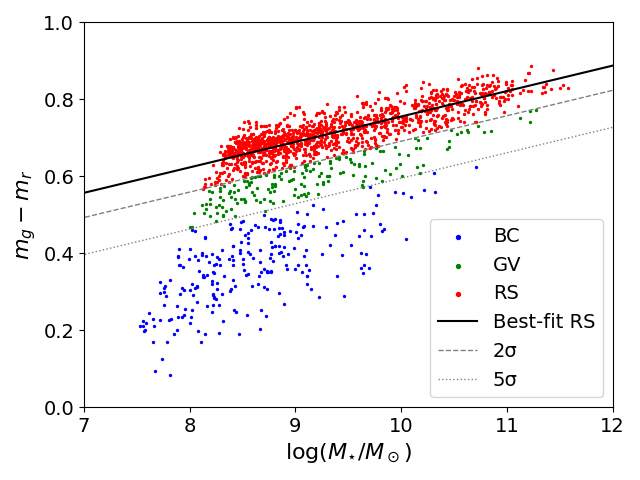
\includegraphics[width=0.9\linewidth]{images/colors_DESI.png}
   \caption{$(m_g-m_r)$ vs stellar mass diagram. The colour of the markers highlights the three colour classes: blue cloud (BC) in blue, red sequence (RS) in red and green valley (GV) in green. The solid line represents the best fit for RS galaxies, the dashed and dotted lines indicate the $2\,\sigma$ and $5\,\sigma$ limit, respectively.}
    \label{fig:colors}
\end{figure}



\subsection{Numerical density profile}
\label{num_density_methods}

The distribution of galaxies in clusters is shaped by that of dark matter, which dominates the total mass of the system and determines the overall gravitational potential. %As a consequence, in dynamically relaxed clusters, we expect the numerical density profile of member galaxies $\nu(r)$ to follow the same functional form as that of the total matter density profile (\textit{e.g.}\,\citealt{Biviano_2003}). 
A widely adopted model to describe the total mass density profiles of gravitationally bound systems, such as galaxy clusters, is the  Navarro-Frenk-White (NFW) model \citep{Navarro_1997}:

\begin{equation}
    \rho_{\rm NFW}(r)=\frac{\rho_{0,_{\rm NFW}}}{(r/r_{\rm s})\, (1+r/r_{\rm s})^2} \, ,
    \label{NFW}
\end{equation}
proportional to $r^{-1}$ in the innermost region and to $r^{-3}$ at large radii. In Eq.~\ref{NFW}, $\rho_0$ is the characteristic density of the cluster and $r_{\rm s}=r_{-2}$ is the scale radius at which the logarithmic derivative of the profile equals $-2$. While initially proposed as a description of dark matter halos in N-body cosmological simulations, the NFW profile has been shown to provide an adequate description of the total mass distribution of clusters (\textit{e.g.} \citealt{Umetsu16, Pizzuti_2025b}). 

%Integrating Eq. \ref{NFW} along the LoS, one recovers the analytic form of the projected Navarro-Frenk-White (pNFW) numerical profile:

%\begin{equation}
% \nu_{\rm NFW}\, (x)= \nu_{0,_{\rm NFW}}  \begin{cases}
%  \frac{\operatorname{arccosh}(1/x)}{\sqrt{1-x^2}} +\ln(\frac{x}{2})    & \text{} x < 1 \\
%  1-\ln2 & \text{} x = 1 \\
%  \frac{\arccos(1/x)}{\sqrt{x^2-1}} +\ln(\frac{x}{2})    & \text{}    x > 1 \, ,
%  \end{cases}
%\end{equation}

%here $x=R/r_\nu$, being $R$ the projected radius and $r_\nu$ the scale radius of the number density profile.
The projection of the NFW profile \citep{bartelmann1996} is found to be also suitable to describe the spatial distribution of cluster members $\nu(r)$ on the plane of the sky (\textit{e.g.} \citealt{Lin_2004, Annunziatella_2014, Sartoris_2020}); however, it is important to note that the scale radius of the number density of galaxies $r_\nu$ is not in general the same as the scale radius $r_{\rm s}$ of the mass profile \citep{Biviano_2006, Budzynski_2012}. In fact, while RS galaxies typically follow a similar distribution to that of dark matter, BC galaxies tend to have a much less concentrated profile, with typical values of $r_\nu^{\rm BC} \sim 4 \, r_\nu^{\rm RS}$ (\textit{e.g.} \citealt{Collister_2005}).

We further consider the Hernquist model (and its projection, \citealt{Hernquist_1990}), which exhibits a faster decline at large radii:
\begin{equation}
    \nu_{Her}(r) \propto \frac{1}{(r/r_{\nu}^{\rm H})\, (1+r/r_{\nu}^{\rm H})^3} \, ,
    \label{Hernquist}
\end{equation}
%Another model that has been proven to accurately reproduce the total mass density profile of galaxy clusters \citep{Maraboli_2025} is the Hernquist model \citep{Hernquist_1990},
%\begin{equation}
%    \rho_{Her}(r)=\frac{\rho_{0,_{Her}}}{(r/r_H)\, (1+r/r_H)^3} \, ,
%    \label{Hernquist}
%\end{equation}
with the characteristic scale $r_\nu^{\rm H}=2\,r_{-2}$ typically two times the corresponding scale radius $r_\nu$ of the projected NFW model.
%Analogue integration of Eq. \ref{Hernquist} along the LoS yields the analytic form of the projected Hernquist (pHer) numerical profile:

%\begin{equation}
% \nu_{Her}\, (x)= \nu_{0,_{Her}}  \begin{cases}
%  \frac{x^2}{1-x^2}\left[\frac{\ln\left(\frac{1+\sqrt{1-x^2}}{x}\right)}{\sqrt{1-x^2}} -1\right]    & \text{} x < 1 \\
%  1/3 & \text{} x = 1 \\
%  \frac{x^2}{1-x^2}\left[\frac{\arccos\left(\frac{1}{x}\right)}{\sqrt{x^2-1}} -1\right]     & \text{}    x > 1 \, ,
%  \end{cases}
%\end{equation}

%\noindent where again $x=\frac{R}{r_\nu}$.

We fit the numerical distribution of member galaxies, required in the kinematic analysis, with both projected models -- NFW and Hernquist -- performing a maximum likelihood fit that does not require the binning of the data \citep{Sarazin_1980, Biviano_2013}, assuming a constant completeness of the sample in the projected radial distance explored. %The validity of this rather strong assumption has been verified in \citet{Pizzuti_2025b} by carrying out a detailed analysis on a few clusters to check thatreasonable variation of the completeness does not provide relevant changes in the reconstructed mass or anisotropy profiles.

The best fit values obtained are $r_\nu = 0.71^{+0.07}_{-0.06} \, \mathrm{Mpc}$ in the case of NFW and $r_\nu^{\rm H} = 1.93^{+0.03}_{-0.46} \, \mathrm{Mpc}$ with Hernquist. %The uncertainties on $r_\nu$ were determined by considering a grid of values around the best-fit estimate and evaluating the difference of $-2\,\ln\mathcal{L}$ from the absolute minimum. This difference follows, with good approximation, a chi-squared distribution with one degree of freedom (Wilks' theorem), used to infer the confidence intervals.  
Both models match the observed numerical distributions adequately well, with no significant differences; as such, during the rest of this work we assume a projected Hernquist model as the reference model for the numerical distribution. %and will keep $r_\nu$ fixed at the corresponding best-fit value of $0.71 \, \mathrm{Mpc}$.
The validity of this choice is assessed in Appendix~\ref{app:A}, where we compare the outcome of \textsc{MG-MAMPOSSt} runs with projected NFW and Hernquist models and we treat the scale radius $r_\nu/r_\nu^{\rm H}$ both as a free and fixed parameter. Fig.~\ref{fig:num_density_pNFW} shows the projected surface density profile of galaxies fitted with both profiles.
%As already mentioned, the two scale radius $r_\nu$ and $r_{\rm s}/r_H$ (depending on the assumed mass model) have to be treated separately, even if the same profile is chosen for both number and mass densities: therefore, even if $r_\nu$ will be used as a fixed input parameter for the dynamical analysis with \textsc{MG-MAMPOSSt}, $r_{\rm s}/r_H$ will be kept as a free parameter, allowing the reconstruction of the total mass profile independently from the member galaxies distribution. 
    

\begin{figure}
    \centering
    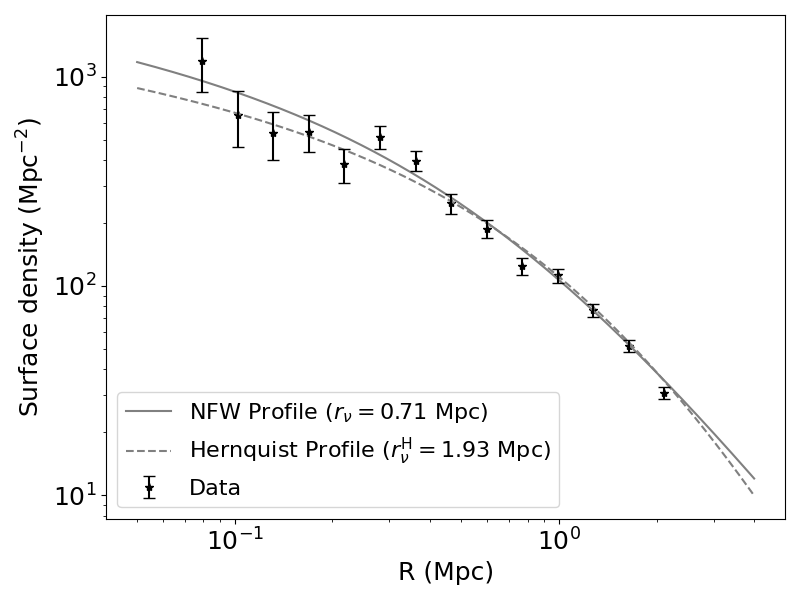
\includegraphics[width=0.9\linewidth]{images/surf_dens_fit_NFWandHer.png}
    \caption{Projected surface density profile of the Coma Cluster fitted with NFW (solid line) and Hernquist (dashed line) models. The error bars correspond to the Poisson uncertainties.}
    \label{fig:num_density_pNFW}
\end{figure}

Since in this work we analyse different subsamples of galaxies based on their colours, we further perform a fit of the numerical profiles of RS, BC, and GV separately, assuming a Hernquist model (see the plot in Appendix \ref{app:B}), finding the scale radii $r_\nu^{\rm RS}=1.64^{+0.02}_{-0.60} \, \mathrm{Mpc}$, $r_\nu^{\rm BC}=5.82^{+3.49}_{-1.80} \, \mathrm{Mpc}$ and $r_\nu^{\rm GV}=12.79 \, \mathrm{Mpc}$ with a lower $1\,\sigma$ uncertainty of $5.71 \, \mathrm{Mpc}$, while the upper bound remains unconstrained due to the particularly flat distribution of GV galaxies in our sample.  It is worth to notice that these results are consistent with the expectation $r_\nu^{\rm BC} \sim 4 \, r_\nu^{\rm RS}$ (\textit{e.g.} \citealt{Collister_2005}). %The extremely diluted distribution of green galaxies reflects the lower statistics and an a-symmetric spatial distribution.  

%A final consideration: previously we have split galaxies into different subsamples, based on their color. Each of them, in principle, has a different numerical distribution, which is reflected, if we assume a pNFW model to be valid in every case, in a different value for $r_\nu$. However, we assume that these changes in the scale radius have a negligible impact on the results and hence keep $r_\nu$ fixed at the standard value for all \textsc{MG-MAMPOSSt} runs, regardless of the considered subsample. A test of this assumption has been performed by fitting the numerical density profile of RS, Gv and BC galaxies (plots in Appendix \ref{app:B}), finding the scale radii $r_\nu^{\rm RS}=0.52^{+0.06}_{-0.05} \, \mathrm{Mpc}$, $r_\nu^{\rm GV}=10.0^{+5.0}_{-5.0} \, \mathrm{Mpc}$ and $r_\nu^{\rm BC}=2.65^{+1.33}_{-0.87} \, \mathrm{Mpc}$, respectively. It is worth to notice that these results are consistent with $r_\nu^{\rm BC} \sim 4 \, r_\nu^{\rm RS}$ (\textit{e.g.} \citealt{Mamon_2019}). Running \textsc{MG-MAMPOSSt} with this new values as input parameters has produced essentially unchanged results, validating our initial assumption.

\subsection{LoS velocity distributions}
\label{subsec:LoS_methods}

As a first diagnostic of the dynamical state of the system, we study the deviations from Gaussianity of the LoS rest-frame velocity distribution of member galaxies \citep{Pizzuti_2020}. This indicator strongly correlates with other commonly used relaxation diagnostics based on X-ray observations, reinforcing its suitability for characterising the global dynamical state of a cluster \citep{Roberts_2018}. As mentioned in Sect.~\ref{sec:intro}, observations and simulations consistently show that in dynamically relaxed systems the distribution of LoS velocities are nearly Gaussian, whereas unrelaxed or disturbed systems exhibit significant departures from Gaussianity \citep{Yahil_1977, Boselli_2006, Ribeiro_2013}. To quantify such deviations, we apply the Anderson-Darling test \citep{Anderson_1952} on the LoS velocity distributions for RS, GV, and BC 
%red sequence, green valley and blue cloud 
subsamples, up to $3$ Mpc. Values of the Anderson-Darling distance $A^2$ coefficient that are above $0.752$ indicate a $\geq 95\% $ confidence that the velocity distribution is inconsistent with a Gaussian.

The LoS velocity distributions for RS, GV, and BC
%red sequence, green valley and blue cloud 
galaxies are shown in Fig.~\ref{fig:vel_LoS}. The three distributions are not significantly different, according to a Kruskal-Wallis test \citep{KW52}, nor are their medians, according to two-by-two comparisons by the Sign test \citep{DM46}. However, the three distributions display different shapes.
The resulting $A^2$ coefficient for RS galaxies is $\sim0.29$, a low value which suggests that orbits are almost completely virialised. On the contrary, BC galaxies exhibit a notable deviation from Gaussianity with $A^2 \sim 1.56$, corresponding to a probability value of less than $1 \%$, due to a skewed distribution towards higher velocities. The excess of high velocities for BC galaxies is clearly visible in Fig.~\ref{fig:phase_space_DESI} at $R<r_{200}$, and it causes a
negative correlation between $R$ and $v_\text{RF}$ (Spearman rank correlation coefficient $r=0.097$, corresponding to a probability of 0.05). No such correlation is present for the RS and GV classes. These characteristics of the BC velocity distribution suggest more elongated orbits for LTGs, which might be infalling towards the cluster centre from a filamentary-like structure at the near-side of the cluster along the LoS. This interesting feature will be addressed specifically in an upcoming paper (paper II), dedicated to substructures and dynamical state.
%and will eventually undergo interactions with the ICM, leading to gas depletion and star formation quenching \citep{Boselli_2006}. 
GV galaxies velocity distribution shows a quite unrelaxed behaviour too, with a coefficient $A^2 \sim 1.27$, lower than that of the BC but significantly higher than that of the RS. As for the full sample, we found a value of $A^2 \sim 0.80$, higher than that of the RS but smaller than that of the GV, which indicates that the overall system is quite far from a full dynamical relaxation state, consistently with the presence of still infalling star forming galaxies.


\begin{figure}
    \centering
    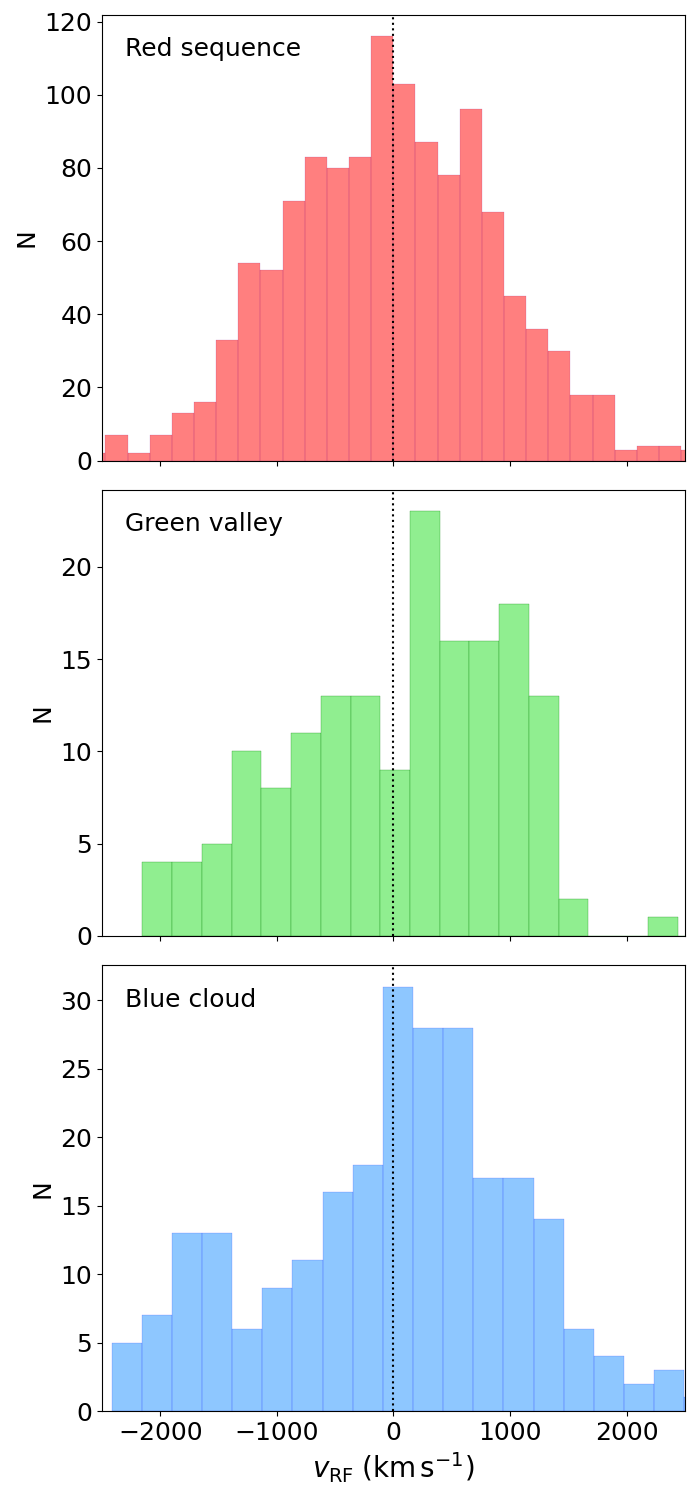
\includegraphics[width=0.8\linewidth]{images/vel_distrib_colors_vertical.png}
    \caption{LoS velocity distributions of RS (upper panel), GV (middle panel) and BC (lower panel) galaxies. The vertical dashed line indicates the average velocity of the cluster. }
    \label{fig:vel_LoS}
\end{figure} 

%\begin{figure*}
 %   \centering
 %   \includegraphics[width=0.3\linewidth]{images/vel_distrib_RS.png}
  %  \includegraphics[width=0.3\linewidth]{images/vel_distrib_GV.png}
  %  \includegraphics[width=0.3\linewidth]{images/vel_distrib_BC.png}
  %  \caption{LoS velocity distributions of red sequence (left panel), green valley (middle panel) and blue cloud (right panel) galaxies. The vertical dashed line indicates the average velocity of the cluster. }
   % \label{fig:vel_LoS}
%\end{figure*} 

\section{Kinematic analysis with MG-MAMPOSSt}
\label{sec:mamposst}

We perform a kinematic analysis of the Coma Cluster member galaxies by means of the \textsc{MG-MAMPOSSt} (Modified Gravity - Modelling Anisotropy and Mass Profiles of Observed Spherical Systems) code of \citet{Pizzuti_2021}, an extended version of the \textsc{MAMPOSSt} algorithm of \cite{Mamon_2013}, which  reconstructs galaxy cluster total mass  and velocity anisotropy profiles in a wide variety of cosmological setups (including $\Lambda$CDM and several modified gravity/dark energy frameworks). 

\textsc{MAMPOSSt} is a way to jointly reconstruct the anisotropy and mass profiles of spherical systems using kinematics of the system's members. In particular, the code assumes dynamical relaxation, spherical symmetry and a shape for the three-dimensional velocity distribution of the tracers of the gravitational potential (\textit{i.e.} cluster member galaxies). Taking as input the p.p.s. dataset $(R,v_\text{RF})$,  \textsc{MAMPOSSt} performs a Maximum Likelihood fit to solve the stationary and spherically symmetric Jeans equation:

\begin{equation}
    \frac{\text{d}[\nu(r) \, \sigma_r^2(r)]}{\text{d}r} + 2\beta(r) \frac{\nu(r) \, \sigma_r^2(r)}{r} = - \nu(r) \frac{\text{d}\Phi(r)}{\text{d}r} \, ,
    \label{eq:jeans}
\end{equation}

\noindent where $\nu(r)$ is the number density profile of galaxies, $\sigma_r(r)$ is the velocity dispersion along the radial direction, $\beta(r)$ is the orbital anisotropy profile and $\Phi(r)$ is the gravitational potential, linked to the dynamical mass profile through the Poisson equation:
\begin{equation}
    \frac{\text{d}\Phi}{\text{d}r} = \frac{G \, M_{\text{dyn}}(r)}{r^2} \, .
\end{equation}
The orbital anisotropy profile $\beta(r)$ is defined as:

\begin{equation}
    \beta(r) = 1 - \frac{\sigma_\theta^2 + \sigma_\phi^2}{2 \,\sigma_r^2} \, ,
\end{equation}
where  $\sigma^2_\theta$ and $\sigma^2_\phi$ are the velocity dispersions along the tangential and azimuthal directions, respectively. This reduces to 

\begin{equation}
    \beta(r) = 1 - \frac{\sigma_\theta^2}{\sigma_r^2} 
    \label{eq:beta_profile}
\end{equation}
in the case that the cluster velocity structure is invariant under rotation about its center, for which $\sigma^2_\theta =\sigma^2_\phi$. Negative values of $\beta(r)$ indicate tangentially-biased orbits, while positive values signify a preference for radial orbits. A value close to $\beta = 0$ indicates isotropic orbits, typical of central regions of dynamically relaxed systems. Previous studies based on observations \citep[\textit{e.g.}][]{Host_2009, Biviano_2013} and simulations \citep[\textit{e.g.}][]{Hansen_2006, Mamon_2010} of galaxy clusters indicate a growing trend with radius for anisotropy, from central isotropy. %In this work, we check this expectation for the Coma Cluster (Sect.~\ref{full_sample_mamposst}) and if there are any substantial differences in the orbits of different galaxy populations (based on their color, see Sect.~\ref{subsec:diff_sample_mamposst}).

%The Jeans equation \eqref{eq:jeans} is commonly used to infer the mass profile of relaxed stellar systems or galaxy clusters. However, its solutions suffer from the so-called 'mass anisotropy degeneracy' \citep[e.g.,][]{Merritt_1987, Lokas_2003, Biviano_2013, Diakogiannis_2014}. This degeneracy arises because the LoS velocity dispersion profile depends not only on the underlying mass distribution, but also on the orbital anisotropy of the tracers, encoded in the anisotropy profile. Different combinations of the mass profile $M(r)$ and the anisotropy profile $\beta(r)$ can reproduce the same observed velocity dispersion profile. As a result, it is not possible to uniquely determine the mass distribution from
%the LoS velocity dispersion profile alone.
%kinematic data alone, unless independent constraints on $\beta(r)$ are available.
%\textsc{MAMPOSSt} overcomes this limitation by using the additional information available from the p.p.s., that is, by estimating 

\textsc{MAMPOSSt} estimates the probability $q\, (R_i, v_i^\text{RF} \, | \, \vec{\theta})$ of
observing the \textit{i}-th tracer of the gravitational potential (e.g. a cluster galaxy) at a projected distance from the cluster centre ($R_i$) and LoS rest-frame velocity ($ v_i^\text{RF}$), given the set of parameters $\vec{\theta}$ defining the models for $M_{\text{dyn}}(r)$ and $\beta(r)$. Other similar approaches have been proposed that use additional information from the observed kinematics beyond the simple velocity dispersion profile, e.g. the kurtosis profile \citep{Lokas02}. The output of the code is the best fit estimate of the parameters $\vec{\theta}$ and the corresponding value of $-\ln \mathcal{L}$, computed as:

\begin{equation}
    -\ln \mathcal{L} = -\sum_{i=1}^{N} \ln  q\, (R_i, v_
{i}^\text{RF} \, | \, \vec{\theta})  \, ,
\end{equation}
where $N$ is the total number of tracers.
%adopting a parametric approach to estimate, at the same time, the mass profile and the anisotropy profile: this reduces degeneracy by incorporating more information and by constraining the models within a well-defined parameter space, at the cost of introducing assumptions about the functional form of both profiles.
The current implementation of \textsc{MG-MAMPOSSt} assumes a 3D Gaussian velocity distribution; despite its simplicity,  this choice has been proven to be valid also when the LoS velocity distribution significantly deviates from Gaussianity \citep{Mamon_2013, Read21}. Refer to \citet{Mamon_2013} for all the expressions regarding the \textsc{MAMPOSSt} procedure.

%Given a parametric expression for $\nu(r),\beta(r)$ and $M_\text{dyn}(r)$ (or, equivalently, the gravitational potential), the code solves the Jeans equation to obtain $\sigma^2_r(r,\vec{\theta})$, being $\vec{\theta}$ the vector of parameters describing the number density, anisotropy and mass models, and computes the probability density
%---------------------------------------------------------------------
%\begin{equation} \label{eq:probdens}
%    g(R,v_{RF}) = \sqrt{\frac{2}{\pi}} \int_R^\infty \frac{r \nu(r)}{\sqrt{r^2 - R^2}} \frac{1}{\sigma_z(r, R)} \exp\left[ -\frac{(v_{RF})^2}{2 \sigma_z^2(r, R)} \right] \, \text{d}r \, ,
%\end{equation}
%---------------------------------------------------------------------
%where $\sigma^2_z(r,R) = \left[ 1 - (R^2/r^2)\,\beta(r) \right]\sigma^2_{r}(r)$ is the velocity dispersion along the LoS. From eq.~\eqref{eq:probdens}, the (log) likelihood is computed as:
%---------------------------------------------------------------------
%\begin{equation}
 %   -\ln \mathcal{L} = -\sum_{i=1}^{N} \ln  q\, (R_i, v_
%{i}^{RF} \, | \, \vec{\theta})  \, ,
%\end{equation}
%---------------------------------------------------------------------
%with $q\, (R, v_{RF} \, | \, \vec{\theta})$ the probability of observing a galaxy at position $(R, v_{RF})$ in the p.p.s. given the model described by the set of parameters $\vec{\theta}$. This is given by:
%---------------------------------------------------------------------
%\begin{equation}
%    q\, (R, v_{RF}) = \frac{2\pi R \, g\, (R, v_{RF})}{N_\text{proj}(R_\text{max})-N_\text{proj}(R_\text{min})} \, ,
%\end{equation}
%---------------------------------------------------------------------
%where $N_\text{proj}(\,R\,)$ is the predicted cumulative number of galaxies within projected radius $R$ from the center, obtained by integrating within the circle of radius $R$ the surface density $\Sigma(R)$ (i.e. the integral of $\nu(r)$ along the LoS). $R_\text{min}$ and $R_\text{max}$ are, respectively, the minimum and maximum projected radii considered in the p.p.s.. The output of the code is the best fit estimate of the parameters $\vec{\theta}$ and the corresponding value of $-\ln \mathcal{L}$.
%we employ a Monte Carlo-Markov Chain (MCMC) module to efficiently explore the parameter space, in which the chain is based on a simple Metropolis-Hastings algorithm with a fixed-step Gaussian random walk. We sample 110000 points and discard the first 10000 as burn-in phase. 

For our kinematic analysis,  we consider a total sample (i.e. BC + RS + GV) of 1324 galaxies out of 1651 members, within a projected radius $R \ge 0.10 \, \mathrm{Mpc}$ and $R \le 2.30 \,\mathrm{Mpc} $ (chosen as $1.1$ times our initial guess for $r_{200}$) from the cluster centre. We exclude the innermost region, as done in many similar works, where cluster dynamics is dominated by the BCG and the mass profile $M_{\rm dyn}(r)$ is likely to deviate from simple profiles that are known from cosmological simulations to adequately describe the distribution of dark matter (e.g. NFW).
Moreover, in Coma the core is dominated by two bright galaxies, namely NGC 4874 and NGC 4889, which  would need a non-trivial modelling of the mass profile.

As for the external regions, at large radii, galaxies are likely to belong to surrounding large-scale structures \citep[\textit{e.g.}][]{Malavasi20}, and are not gravitationally bound to the cluster, so that they cannot be used as tracers of the cluster potential in the dynamical equilibrium configuration. To ensure the robustness of the mass and anisotropy reconstruction, we performed additional runs of \textsc{MG-MAMPOSSt} varying the inner and outer radius, changing the centre and the velocity rest frame of the cluster. The results of these tests are reported in Sect.~\ref{subsec:syst}.

%outer radius by $\sim 30\%$; we confirm that the change in the results is negligible compared to statistical uncertainties (see Fig.~\ref{fig:mass}).

We explore four different mass models for the total mass of the Coma Cluster in the kinematic analysis. We have employed the classical NFW (see Eq. \ref{NFW}), whose total mass can be written as 
%---------------------------------------------------------------------
\begin{equation}
         M_\text{NFW}(r) = M_{200}\frac{\text{ln}(1+r/r_\text{s}) - \frac{r/r_\text{s}}{(1+r/r_\text{s} )}  }{\text{ln}(1+c_{200}) - \frac{c_{200}}{(1+c_{200} )}  }\,,
        \end{equation}
%---------------------------------------------------------------------
where $c_{200} = r_{200}/r_{\rm s}$ is called 'concentration', together with its generalized version gNFW~\citep{Nagai2007}:

\begin{equation}
    \small
    \begin{aligned}
    M_{\text{gNFW}}(r)=\; & M_{200} \, (r/r_{200})^{3-\alpha} \\ & \times  \frac{\prescript{}{2}F_1(3-\alpha,3-\alpha,4-\alpha,-r/r_{\rm s})}{\prescript{}{2}F_1(3-\alpha,3-\alpha,4-\alpha,-r_{200}/r_{\rm s})} \, ,
    \end{aligned}
    \label{gNFW}
\end{equation}
where $\prescript{}{2}F_1(a,b,c,x)$ is the ordinary (Gaussian) hypergeometric function \citep[\textit{e.g.}][]{Mamon_2019}. This model adds an extra free parameter $\alpha$ that controls the slope. Note that, instead of the characteristic density $\rho_0$, we consider the virial radius $r_{200}$ as a free parameter of all the profiles. 

The Hernquist \citep{Hernquist_1990},
%---------------------------------------------------------------------
    \begin{equation}
         M_\text{Her}(r) = M_{200}\frac{(r_{200}+ r_\text{H})^2}{r_\text{200}^2}\frac{ r^2}{(r+ r_\text{H})^2}\,,\label{eq:her}
    \end{equation}
%---------------------------------------------------------------------
and the Burkert \citep{Burkert_1995} models:
%---------------------------------------------------------------------
    \begin{equation}
    \small
         M_\text{Bur}(r) = M_{200}\frac{\text{ln}\big[1+(r/r_\text{B})^2\big] +  2\,\text{ln}(1+r/r_\text{B}) - 2\,\text{arctan}(r/r_\text{B}) }{\text{ln}\big[1+(c_{\rm B})^2\big] +  2\,\text{ln}(1+c_{\rm B}) - 2\,\text{arctan}(c_{\rm B})}\,,\label{eq:bur}
    \end{equation}
%---------------------------------------------------------------------
have been further adopted in the analysis. In eq.~\eqref{eq:her}, $r_{\rm H} = 2 \, r_{-2}$, while in eq.~\eqref{eq:bur}, $r_{\rm B} \simeq 0.657 \, r_{-2}$ and $c_{\rm B} = r_{200}/r_{\rm B}$. The Burkert profile has the same asymptotic behaviour as NFW but exhibits a core in the centre ($\rho \propto \mathrm{const}$) rather than a cusp, and a sharper transition from slope 0 to slope 3 than NFW. We will denote with $r_\rho$ the general scale radius, which takes the form of $r_{\rm s}$, $r_{\rm H}$ or $r_{\rm B}$ depending on the mass model used.

%, the expression for the mass profiles can be written as \citep{Mamon_2013}:
%\begin{equation}
%    M(r)=M(r_\rho)\frac{\hat{M}(r/r_\rho)}{\hat{M}(1)} \, ,
%    \label{eq:mass_profiles}
%\end{equation}

%\noindent where

%\begin{equation}
% \hat{M} (x)=  \begin{cases} \ln(x+1) -
%  \frac{x}{x+1}    & \text{} (\text{NFW}) \\
%  \left(\frac{x}{x+1}\right)^2 & \text{} (\text{Hernquist}) \\
%  \ln[(x+1)^2\,(x^2+1)] -2\, \arctan(x)    & \text{}    (\text{Burkert}) \, .
%  \end{cases}
%\end{equation}


For the anisotropy profile, we consider two general models, namely a generalized version of the  
\citet[][gT, hereafter]{Tiret+07} profile,

\begin{equation}
    \beta_{gT}(r)=\beta_0 +(\beta_\infty-\beta_0)\, \frac{r}{r +r_\beta} \, ,
    \label{Tiret}
\end{equation}

\noindent and the generalized Osipkov-Merritt model \citep{Osipkov_1979, Merritt_1985} (gOM),

\begin{equation}
    \beta_{gOM}(r)=\beta_0 +(\beta_\infty-\beta_0)\, \frac{r^2}{r^2 +r_\beta^2} \, .
    \label{Osipkov-Merritt}
\end{equation}
where $\beta_0$ and $\beta_\infty$ are the anisotropies at the centre and large radii, respectively, and $r_\beta$ is a characteristic radius. These profiles capture a large variety of orbits from the innermost region to the outskirts of a cluster. Note that, as done in previous works (\textit{e.g.} \citealt{Mamon_2019,Biviano24}), we assume $r_\beta= r_{-2}$ of the mass profile, a reasonable assumption to avoid an extra free parameter in the fit, which, in our case, would be largely unconstrained.

The high-quality performances of the DESI instrument results in very small uncertainties on the LoS velocities (see \citealt{DESI_DR1}), which are $<10$ km/s for emission line galaxies and between 5-30 km/s for passive galaxies, as a function of magnitude. As such, in our analysis we adopt a constant uncertainty of $40 \, \mathrm{km \, s^{-1}}$, as a conservative safe upper limit for all the galaxies in our sample.

\textsc{MG-MAMPOSSt} is equipped with a Monte Carlo-Markov Chain (MCMC) module to efficiently explore the parameter space, based on a simple Metropolis-Hastings algorithm with a fixed-step Gaussian random walk; the code can handle both flat and Gaussian priors on the free parameters. In the following, we sample 110000 points and discard the first 10000 as burn-in phase. 
This number of steps is sufficient to ensure the convergence of the chains; checks has been performed by previous studies in similar frameworks \citep{Pizzuti_2024,Biviano25}, where the Gelman-Rubin diagnostic coefficients $\hat{R}$ \citep{Gelman_1992} have been computed after performing 5 chains on each run, satisfying the requirement of $\hat{R}<1.1$. Each chain takes $\lesssim 1 $ hour to be completed.
The details of the analysis and the results of \textsc{MG-MAMPOSSt} on the various subsamples of member galaxies are presented and discussed in the next Section.
%The analysis with \textsc{MG-MAMPOSSt} of the full sample of galaxies is presented in Sect.~\ref{full_sample_mamposst}, while the study of different subsamples can be found in Sect.~\ref{subsec:diff_sample_mamposst}. 

%%%%%%%%%%%% commentato fin qui, ABi, 29-XII-2025

\section{Results \& Discussion}
\label{results}




\subsection{Mass and anisotropy profiles analysis}
\label{full_sample_mamposst}

The strategy we adopted to robustly model the mass and orbital anisotropy profiles of the Coma Cluster is the following: first, we performed a run of \textsc{MG-MAMPOSSt} on the p.p.s. of the mixed sample of 1324 galaxies, thus using all the RS, GV, and BC populations as tracers of the gravitational potential. This methodology has been used several times in the literature and it has been shown to work quite well when comparing to independent mass estimates \citep[\textit{e.g.}][]{Sartoris_2020, Biviano_2013, Biviano_2023}. Then, we split the sample by colour class and we ran \textsc{MG-MAMPOSSt} separately on each population to infer the mass profiles predicted by RS, GV, and BC galaxies, respectively. The colour-dependent posterior distributions of the mass profile parameters were then combined to get the final constraints on the cluster mass profile. This procedure allowed us to check whether the two independent Bayesian estimates are in agreement within each other, and provide further support to the viability of mixing different galaxy populations to reconstruct the total gravitational potential of clusters. 
\medskip

%We first \textbf{ran} \textsc{MG-MAMPOSSt} for all the combination of mass, anisotropy and number density models considering the p.p.s. of the \textbf{full} sample of 1347 galaxies, \textbf{thus assuming that the RS, GV and BC populations have the same $\beta(r)$}.
We considered two free parameters for the mass profile, $r_{200}$ and $r_\rho$ -- in the case of NFW, Burkert and Hernquist models. We also treated the scale radius of the numerical density profile $r_\nu^H$ as a free parameter, assuming a projected Hernquist model (see Appendix \ref{app:A}). In addition, letting $\mathcal{A}=\sigma_r /\sigma_\theta = (1-\beta)^{-1/2}$, we adopted two free parameters for the velocity anisotropy: $\mathcal{A}_0$ and $\mathcal{A_{\infty}}$ for the inner and outer values, respectively. This definition rescales the range $-\infty < \beta < 1$ into $0 < \mathcal{A} < \infty$, preventing numerical issues at $\beta \sim 1$. For the gNFW model, the additional exponent $\alpha$ was further optimized within the fit. The assumed priors are listed in Table \ref{tab:priors_flat}: they are flat for every parameter and uninformative for each of them except for $r_\nu^H$, for which we adopted informative priors based on the best fit values discussed in Sect. \ref{num_density_methods}.

%--------------------------------------------------------
\begin{table}
\centering
\renewcommand{\arraystretch}{1.1}
\caption{Assumed priors for \textsc{MG-MAMPOSSt} runs with mixed components.}
\begin{tabular}{lccccc}
\hline
{Parameter} & {Prior type} & {Min} & {Max} \\%& {Initial guess}\\
\hline
       
       $r_{200} \, (\mathrm{Mpc)}$ & log-Flat & $\log_{10}(1.0/{\rm Mpc})$ & $\log_{10}(3.0/{\rm Mpc})$ \\%& 2.1 \\
       $r_{\rho} \, (\mathrm{Mpc)}$ & log-Flat & $\log_{10}(0.2/{\rm Mpc})$ & $\log_{10}(5.0/{\rm Mpc})$ \\%& 0.5\\
       $r_\nu^{\rm H} \, (\mathrm{Mpc)}$ & log-Flat & $\log_{10}(1.4/{\rm Mpc})$ & $\log_{10}(2.1/{\rm Mpc})$ \\%& 0.5\\
       $\mathcal{A}_0$ & Flat & 0.5 & 5.0 \\%& 1.2\\
       $\mathcal{A}_\infty$ & Flat & 0.5 & 5.0 \\% & 3.0\\
       $\alpha$ & Flat & 0.1 & 1.9 \\ %& 1.0\\     
\hline
\end{tabular}
\caption*{\footnotesize \textbf{Notes.} $\alpha$ is a free parameter only when the gNFW model is used for the mass density profile.}
%\caption*{\footnotesize{Notes:}}{$\alpha$ is a free parameter only when the gNFW model is used for the mass density profile.}
\label{tab:priors_flat}
\end{table}
%--------------------------------------------------------

%The estimates of the virial mass $M_{200}$ and their errors are shown in Fig.~\ref{fig:mass}.
Different combinations of $M_{\rm dyn}(r)$ and $\beta(r)$ models provided mass estimates in agreement within the uncertainties, which indicates robustness of the results. Since some runs involved a different number of galaxies or free parameters, we used the Bayesian Information Criterion (BIC) and the Akaike Information Criterion (AIC) to provide a rough estimate of the performance of each combination of models. The BIC criterion is defined as:
%=======================================================
\begin{equation}
    \text{BIC} = k \, \ln(N) - 2 \, \ln\mathcal{L} \, ,
    \label{eq:BIC}
\end{equation}
%=======================================================
where $k$ is the number of free parameters in the run, $N$ is the total number of tracers used in the analysis, in our case the member galaxies, and $\ln\mathcal{L}$ is the best fit log-likelihood. Lower BIC values indicate preferred models: in fact, the penalty term $k \, \ln(N)$ increases with both the number of parameters and the number of data points, discouraging overly complex models unless they provide a significantly better fit. As $k$ increases, the model gains flexibility and typically achieves a higher (less negative) log-likelihood, but this comes at the cost of a larger penalty. Conversely, a model with fewer free parameters is rewarded by a smaller penalty. Similarly, the AIC criterion is defined as:

\begin{equation}
    \text{AIC} = 2\,k \, - 2 \, \ln\mathcal{L} \, ,
    \label{eq:AIC}
\end{equation}
which, in our case, reduces the penalty caused by the increasing of the number of free parameters. In this analysis, only the runs assuming a gNFW model for the mass density profile present an extra free parameter; therefore, a comparison of the BIC/AIC parameter between runs not using gNFW and considering the same number of galaxies in the analysis essentially consists in checking the difference in the respective log-likelihoods.  

The resulting BIC and AIC values suggest that the NFW model for the mass profile is favoured with respect to the Burkert and Hernquist models, and the gOM anisotropy model is slightly better than the gT model, but differences in the Bayesian evidence values are negligible. Therefore, we considered as the reference estimates for the parameters with mixed components those of the NFW gOM run, reported in the corresponding column of Table \ref{tab:diff_samples_results}. Note that the best fit values reported in every Table of this paper correspond to the maximum likelihood values. %$M_{200} = 1.12_{-0.08}^{+0.14} ({\rm stat}) \pm 0.10 ({\rm syst}) \,\times 10^{15} \, M_\odot $ at 1$\sigma$, where the systematic uncertainties take into account the variation of the best fit due to different choices of the \textbf{mass and anisotropy models assumed for the mixed sample. 
 
For the mixed-population run, we plot the reconstructed mass profile along with its $1\,\sigma$ and $2\,\sigma$ uncertainty regions as the purple dashed and dotted lines, respectively, in Fig.~\ref{fig:mass_profile} (left panel). The anisotropy profile, shown in Fig.~\ref{fig:anis_profile}, indicates the presence of radial orbits both in the outer and in the inner regions of the system, %and orbits closer to isotropy in the innermost part, 
 with only a slight variation with radius. %This behaviour is consistent with galaxies in the inner regions having reached more advanced stages of virialization, whereas in the outer regions 
The prevalence of radial orbits reflects 
%the ongoing accretion of still infalling galaxies. 
the presence of a population of recently accreted galaxies from the surrounding large-scale structure.

%The marginal distributions for the free parameters of the NFW+gOM model are presented in Fig.~\ref{fig:triangle_full}. 
%As mentioned above, the central anisotropy is in agreement with $\mathcal{A}_0 = 1$, corresponding to isotropic orbits $\beta = 0$, while the anisotropy at large radii prefers larger values $\beta > 0$.
It is worth to point out that our constraints on $r_{\rm s}$ are consistent with the concentration values found by \citet{Gavazzi_2009}.
%and that the $r_{\rm s}$ values of the mass and RS galaxy distributions are almost identical.
When running with the gNFW, the inner slope of the mass density profile is estimated as $\alpha=1.71_{-0.39}^{+0.16}$, at the cost of a totally unconstrained scale radius of the mass profile. The BIC for this run is 7 units higher (worse) than the reference run, but the difference reduces to only 2 units when using the AIC criterion.

We then ran \textsc{MG-MAMPOSSt} on the p.p.s. of the different colour classes. Based on the analysis performed with the mixed components, here we kept the NFW and the gOM as the reference mass density and anisotropy profile models. The employed priors were the same as those used for the mixed sample analysis (Table \ref{tab:priors_flat}), with the exception of $r_\nu^H$ for which priors were adapted for each class following the results of Sect.~\ref{num_density_methods}. The number of galaxies between $0.10 \,\mathrm{Mpc}$ and $2.30 \,\mathrm{Mpc}$ -- the minimum and maximum radii considered for the reference analysis -- is 1030 for the RS, 129 for the GV, and 152 for the BC. The estimates of the free parameters, for each of the three populations, are reported in the corresponding columns of Table \ref{tab:diff_samples_results}. 

As expected, the dynamics is completely dominated by the RS galaxies, producing a profile in excellent agreement with that obtained from the mixed sample, as further shown by the red solid curve in Fig.~\ref{fig:mass_profile} (left). While the analysis of the GV sample tends to underestimate the total mass at all radii, the BC galaxies favour a less concentrated and more massive cluster, supporting the idea that they are farther away from dynamical equilibrium.


When combining the three marginalised posterior distributions $\ln P_\text{joint}(r_{200},r_\text{s}) = \sum_i  P_i(r_{200},r_\text{s})$, with $i = $ RS, BC, GV, we obtain $M_{200} = 1.08_{-0.09}^{+0.08}~({\rm stat}) \pm 0.09~({\rm syst}) \times 10^{15} \, \mathrm{M}_\odot $, corresponding to $r_{200}=2.12 \pm 0.06~({\rm stat})\pm0.07 ~({\rm syst}) \, \mathrm{Mpc}$ and a scale radius for the mass profile $r_{\rm s} =0.48^{+0.27}_{-0.13} \, \mathrm{Mpc}$. The systematic uncertainties take into account the variation of the best fit due to different choices of the mass and anisotropy models, as well as the variations of projected radial range considered, cluster centre and velocity rest frame (see Sect.~\ref{subsec:syst}). The mass profile and the corresponding $1$ and $2\,\sigma$ regions are shown as grey shaded areas in the left panel of Fig.~\ref{fig:mass_profile} (left). The right panel of the same Figure displays the relative ratio between ours and other estimates from the literature for the total mass profile of the cluster. Overall, we found a general good agreement among different mass profiles within uncertainties, with the largest deviations found near the centre. The weak lensing analysis of \cite{Gavazzi_2009} predicts a lower cluster mass, but still in agreement with our value within the $1\,\sigma$ region. For a comparison between our best virial mass measurement and those coming from more recent studies, see also Fig.~\ref{fig:mass_compare} and the discussion in Sect.~\ref{sec:conclusions}. %This is in agreement with both weak lensing studies in \citet{Cha_2025} and \citet{Gavazzi_2009}, as well as with X-ray+SZ effect analysis in \citet{Mirakhor_2020} and with virial theorem estimate in \citet{Benisty25}. Meanwhile, machine learning result in \citet{Ho_2022} is a bit higher and caustics method value in \citet{Benisty25} is a bit lower than ours (see the discussion in Sect.~\ref{sec:conclusions}, Fig.~\ref{fig:mass_compare}). Also the virial radius estimate of $r_{200}=2.07_{-0.06}^{+0.07} \, \mathrm{Mpc}$ is consistent with the estimate given in \citet{Boselli_2006}.

%--------------------------------------------------------
\begin{table*}
\centering
\caption{Best fit parameters for the runs with mixed and separated components.}
\renewcommand{\arraystretch}{1.3}
\begin{tabular}{lccccc}
\hline
Parameter & Mixed & RS & {GV} & {BC} & Joint \\
\hline
       
       $r_{200} \, (\mathrm{Mpc})$ & $2.14_{-0.05}^{+0.09}$ & $2.06_{-0.05}^{+0.07}$ & $1.57_{-0.18}^{+0.48}$ & $2.55_{-0.44}^{+0.21}$ & $2.12\pm 0.06$ \\
       $r_{\rm s} \, (\mathrm{Mpc})$ & $0.70_{-0.30}^{+0.22}$ & $0.61_{-0.37}^{+0.02}$ & $0.83_{-0.62}^{+0.85}$ & $2.42_{-2.18}^{+0.05}$ & $0.48_{-0.13}^{+0.27}$ \\
       $r_\nu^{\rm H} \, (\mathrm{Mpc})$ & $1.70_{-0.13}^{+0.11}$ & $1.27_{-0.08}^{+0.12}$ & $7.40_{-2.48}^{+2.60}$ & $5.17_{-1.72}^{+1.32}$ & / \\
       $\mathcal{A}_0$ & $1.10_{-0.33}^{+0.65}$ &
       $1.00_{-0.30}^{+0.68}$ & $0.81_{-0.25}^{+1.22}$ & $1.78_{-0.86}^{+0.79}$ & / \\
       $\mathcal{A}_\infty$ & $1.46_{-0.58}^{+0.20}$ & $1.60_{-0.58}^{+0.02}$ & $1.89_{-0.73}^{+1.44}$ & $0.99_{-0.29}^{+0.78}$ & / \\
          
\hline
\end{tabular}
\caption*{\footnotesize \textbf{Notes.} The employed mass and anisotropy models are NFW and gOM, respectively. The assumed priors, for these runs, are broad and flat, except for $r_\nu^{\rm H}$, for which we considered informative priors based on the best fit values discussed in Sect. \ref{num_density_methods}.}
\label{tab:diff_samples_results}
\end{table*}
%--------------------------------------------------------


Finally, we performed an additional run to estimate the diffuse dark matter mass profile of the cluster at $r> 0.10$ Mpc. We considered the total (spherical) gas mass $M_\text{\rm gas}(r)$ estimated from the electron density profile \citep{Mirakhor_2020} and the total stellar mass in galaxies.
From the cumulative projected stellar mass distribution $M_{*}(R)$ we obtained the three-dimensional stellar mass profile by fitting a Hernquist model, similarly to what done for the number density distribution, and assigning weights to each galaxy proportional to their mass. 

The \textsc{MG-MAMPOSSt} code was then applied to fit a multi-component mass model as
\begin{equation}\label{eq:multic}
    M_\text{\rm tot}(r) = M_\text{\rm gas}(r) + M_{*}(r) + M_\text{\rm DM}(r)\,,
\end{equation}
where $M_\text{\rm DM}(r)$ is the DM distribution, parametrised as a gNFW model. The uncertainties on the stellar mass profile in galaxies and on the gas mass profile were accounted by first maximum-likelihood-fitting a Hernquist model and a $\beta$-model to the galaxies and gas data, respectively, and using the resulting covariance matrix as a multi-variate Gaussian input prior on the corresponding $M_{*}(r),\,M_\text{\rm gas}(r)$ in the \text{MG-MAMPOSSt} analysis.
%Note that a significant fraction of the baryonic distribution in the cluster center is given by the BCG(s) mass profile. In Coma the core is dominated by two bright galaxies, namely NGC 4874 and NGC 4889, which  need a non-trivial modelling of the mass profile. As such, we exclude the central region 
%in the  in a multi-component fashion, the central mass profile $M_\text{BCG}(r)$, associated with the BCG(s), has also to be accounted. However, the contribution of the shape of such profile to the total matter distribution is relevant only for very small radii ($r \lesssim 50$ kpc, see \textit{e.g.}~\citealt{Biviano:2023oyf}); moreover, in Coma the core is dominated by two bright galaxies, namely NGC 4874 and NGC 4889, which  need a non-trivial modelling of the mass profile. %As such, we consider a 'nuisance' Jaffe model,
%\begin{equation}
%    M_\text{BCG}(r) = \frac{M_0\,(r/r_j)}{1+ r/r_j}\,,
%\end{equation}
%with $M_0$ and $r_j$ free parameters in the fit, encoding our ignorance about the central mass distribution. 

The resulting mass profiles are shown in Fig. \ref{fig:multicompoent} of Appendix \ref{app:mc}. The dark matter dominates at all radii, with a corresponding virial mass $M_{200}^{\rm DM} = 8.6^{+1.2}_{-0.8} \times 10^{14} \, \text{M}_\odot$. The total mass at $r= 2.12$ Mpc, our best fit value for the virial radius, is found to be $M_{\rm tot} = M_{\rm DM}+M_{\rm gas}+M_{*} = (1.09\pm{0.10})\times 10^{15} \,\text{M}_\odot$ in excellent agreement with the single-profile estimates. With this multicomponent approach we can further estimate the value of the baryon fraction as  $f_b \equiv 1- M_{\rm DM}/M_{\rm tot} =  0.15 \pm 0.02$ at $r = 2.12$ Mpc, consistent with the cosmological value of $\Omega_b/\Omega_m$ (\textit{e.g.} \citealt{Krolewski2025}).


%$\alpha=1.11^{+0.70}_{-0.34}$ at 1$\sigma$, which is consistent with the classical NFW model ($\alpha=1$).

%'Larger' and 'smaller' refers to the number of galaxies considered: the standard case considers galaxies up to $2.29 \, \text{Mpc}$ (1359 galaxies), the 'larger' considers galaxies up to $2.50 \, \text{Mpc}$ (1422 galaxies) and the 'smaller' considers galaxies up to $2.2 \, \text{Mpc}$ (1285 galaxies).
%==============================================================
%\begin{figure}
%    \centering
 %   \includegraphics[width=0.9\linewidth]{images/M200_intervals.png}
    %\includegraphics[width=0.8\linewidth]{images/mamposst/Fig.~2025-11-12 184354 (0).png}
 %   \caption{$M_{200}$ estimates and confidence intervals ($1$ and $2\,\sigma$) for the different mixed population runs.  'Larger': galaxies up to $2.60 \, \text{Mpc}$ (1413). 'Smaller': galaxies up to $1.80 \, \text{Mpc}$ (1273 galaxies). Under each bar, the BIC values are displayed. In all runs, the pNFW model is assumed for the number density profile.} %Bottom panel: Normalized probability distribution for $M_{200}$ in NFW gOM run. Dark and light regions indicate $1\,\sigma$ and $2\,\sigma$ confidence intervals.}
  %  \label{fig:mass}
%\end{figure}
%==============================================================
%\begin{figure}
%    \centering
%    \includegraphics[width=0.9\linewidth]{images/mamposst/Figure 2025-11-12 184354 (0).png}
%    \caption{Normalized probability distribution for $M_{200}$ in NFW gOM run. Dark and light regions indicate $1\,\sigma$ and $2\,\sigma$ confidence intervals.}
%    \label{fig:probab_mass}
%\end{figure}

\begin{figure*}
    \centering
    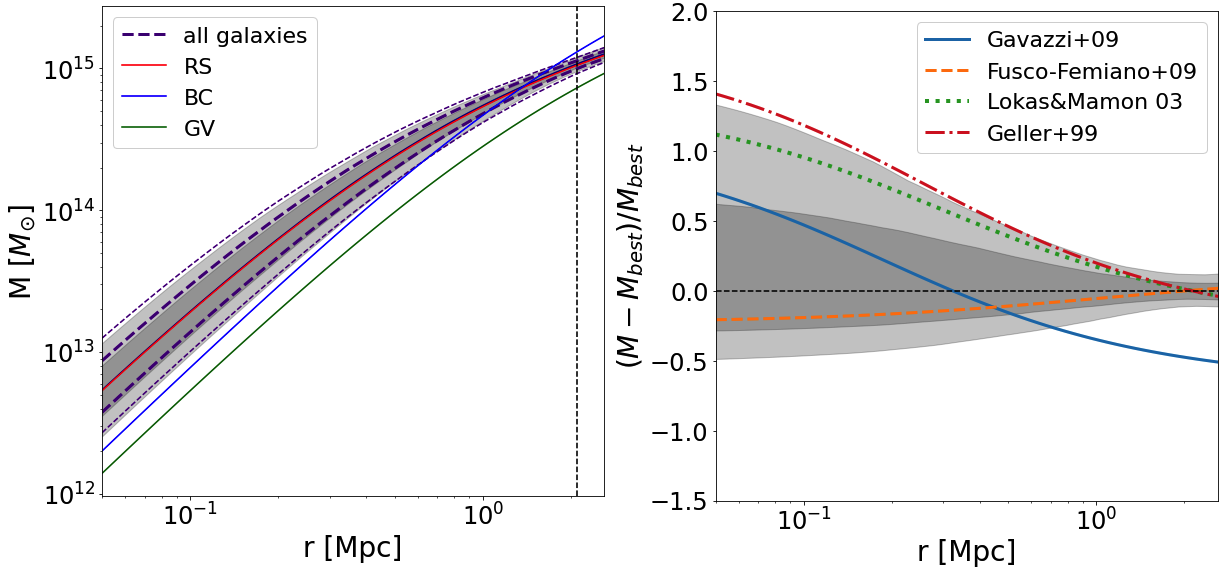
\includegraphics[width=0.85\textwidth]{images/massAndComparisons.png}
    \caption{\textit{Left}: Estimated mass profiles in the \textsc{MG-MAMPOSSt} runs for the mixed components (1 and $2\,\sigma$ regions delimited by purple dashed lines), separated colour classes (RS in red, GV in green, BC in blue) and produced by the joint likelihood (1 and $2\,\sigma$ regions coloured in dark and light grey, respectively, and vertical dashed line corresponding to the virial radius). \textit{Right}: Relative ratio between our best fit $M_{best}(r)$ and other estimates of the full mass profile of Coma from the literature. Blue solid curve: \cite{Gavazzi_2009} (from weak lensing analyses). Orange dashed line: \cite{Fusco2009} (from an X-ray data). Green dotted line: \cite{Lokas_2003}, and red dot-dashed curve: \cite{Geller1999} (both from kinematics analyses). Dark and light grey shadings indicate 1 and $2\,\sigma$ confidence regions on our best fit $M_{best}(r)$. Confidence regions on the literature $M(r)$ are not shown for the sake of clarity.}
    \label{fig:mass_profile}
\end{figure*}

\begin{figure}
    \centering
    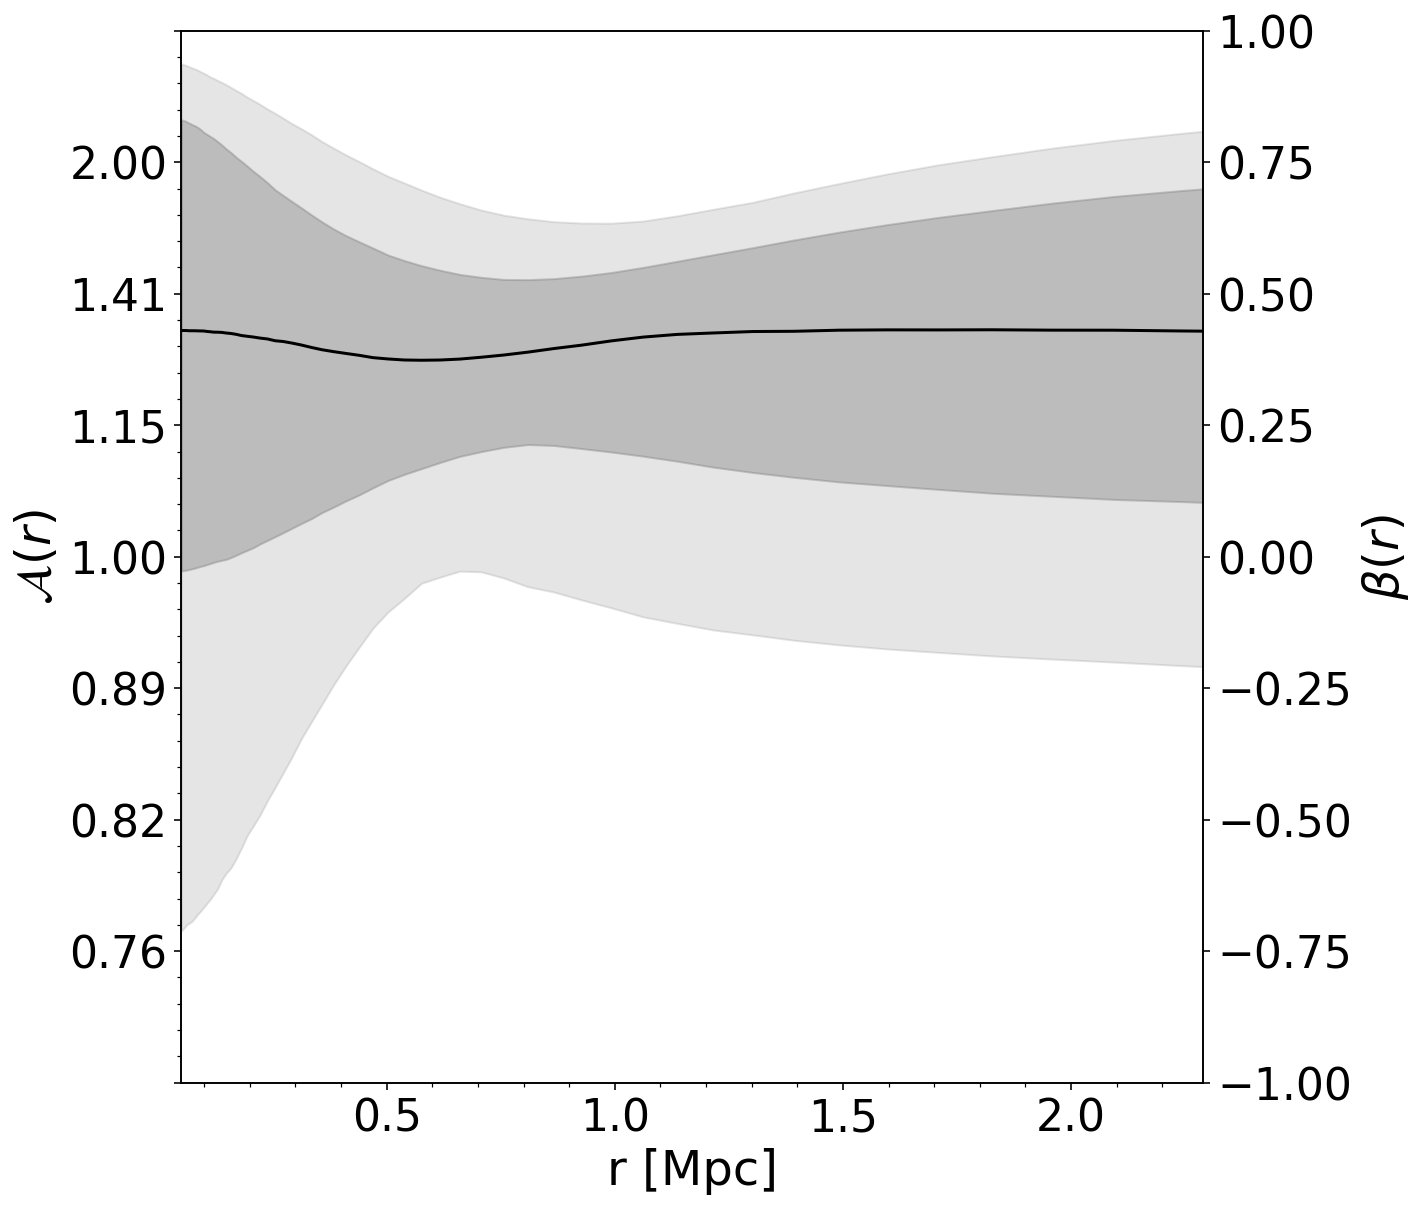
\includegraphics[width=0.8\columnwidth]{images/mamposst/full_anis.png}
    \caption{Estimated anisotropy profile in the \textsc{MG-MAMPOSSt} run for the mixed components with the NFW mass model and gOM anisotropy model. The solid curve is the median profile of the MCMC chain.}
    \label{fig:anis_profile}
\end{figure}

%\begin{figure}
%    \centering
%    \includegraphics[width=0.8\linewidth]{images/mamposst/Figure 2025-11-12 184354 (1).png}
%    \caption{Marginal 2D and 1D distributions for free parameters in NFW gOM run. Black and grey regions mark $1\,\sigma$ and $2\,\sigma$ confidence intervals.}
%    \label{fig:triangle_full}
%\end{figure} 



\subsection{Robustness of mass-orbital modelling}
\label{subsec:syst}

The \textsc{MG-MAMPOSSt} procedure of modelling the mass and orbital profiles of complex systems such as the Coma Cluster produces results that are inevitably depending on several choices and assumptions, whose validity and robustness must therefore be assessed. First of all, one has to assemble the input p.p.s. sample of member galaxies, which, even after the removal of interlopers, is dependent on two main variables:

\begin{enumerate}
    \item[\textit{i)}] The coordinate centre of the cluster, which we located at (RA=194.90 deg, DEC = 27.96 deg), the position of NGC 4874.
    
    \item[\textit{ii)}] The LoS velocity of the rest frame of the cluster, chosen as the biweight mean LoS velocity of its members. 
    
\end{enumerate}    
%---------------------------------------------
The input parametrisations of the mass and anisotropy profiles (see Sect. \ref{full_sample_mamposst}), as well as for the numerical density profile (see Sect. \ref{num_density_methods} and Appendix \ref{app:A}), with their relative priors choice, introduce additional potential sources of uncertainty.

The projected radial range within which galaxies are considered in the fit plays a fundamental role. This depends on:

\begin{enumerate}
    \item[\textit{iii)}] the minimum projected radius, which we chose to be 100 kpc, in order to exclude the innermost region where dynamics is dominated by NGC 4874 and NGC 4889.
    
    \item[\textit{iv)}] the maximum projected radius, which we chose to be 2.30 Mpc, in order to exclude the outer regions, where we cannot ensure dynamical equilibrium. 
    
\end{enumerate} 
%-----------------------------------------
In this Section we want to verify that reasonable variations of the choices of \textit{i)--iv)} lead to results that are within the uncertainties of our reference analysis of Sect. \ref{full_sample_mamposst}. We therefore ran \textsc{MG-MAMPOSSt} again to perform the following tests:

\begin{enumerate}

    \item[\textit{i)}] We moved the coordinate centre of the cluster to the position of NGC 4889 (RA=195.03 deg, DEC=27.98 deg) and to the position of the X-ray peak of emission (RA=194.94 deg, DEC=27.95 deg) \citep{Sato_2011}.
    
    \item[\textit{ii)}] We shifted he LoS velocity of the rest frame of the cluster to the average LoS velocity of RS (which is lower by $\sim 20$ km/s), GV, or BC galaxies (which is higher by $\sim 53$ and $\sim 4$ km/s, respectively). 

    \item[\textit{iii)}] We changed the minimum projected radius to both 50 kpc and 200 kpc.
    
    \item[\textit{iv)}] We changed the maximum projected radius to 1.8 Mpc, 2.6 Mpc and 2.9 Mpc.
    
\end{enumerate} 
%------------------------------------
For these runs we used the same priors of Table \ref{tab:priors_flat} to not introduce other differences that could invalidate the tests. The comparison of the best fit estimates of $r_{200}$ and $r_{\rm s}$ is shown in Fig.~\ref{fig:r200-rs-comparison}. All the results are fully in agreement with each other: the largest differences for $r_{200}$ are observed when changing the maximum radius considered, producing a variation of $\sim 5\%$ and for $r_{\rm s}$ when shifting to the GV rest frame, causing a $\sim 30\%$ variation of the best fit, still well within the much larger uncertainties of $r_{\rm s}$ with respect to $r_{200}$.

Fig.~\ref{fig:relative_anis} shows the relative variation of the anisotropy profiles produced by these runs with respect to the reference profile of Fig.~\ref{fig:anis_profile}: all the profiles are well within the $1\,\sigma$ uncertainty regions of the reference run. We therefore conclude that the mass-orbital modelling of Coma with \textsc{MG-MAMPOSSt} is very robust and only slightly affected by systematics.



\begin{figure*}
    \centering
    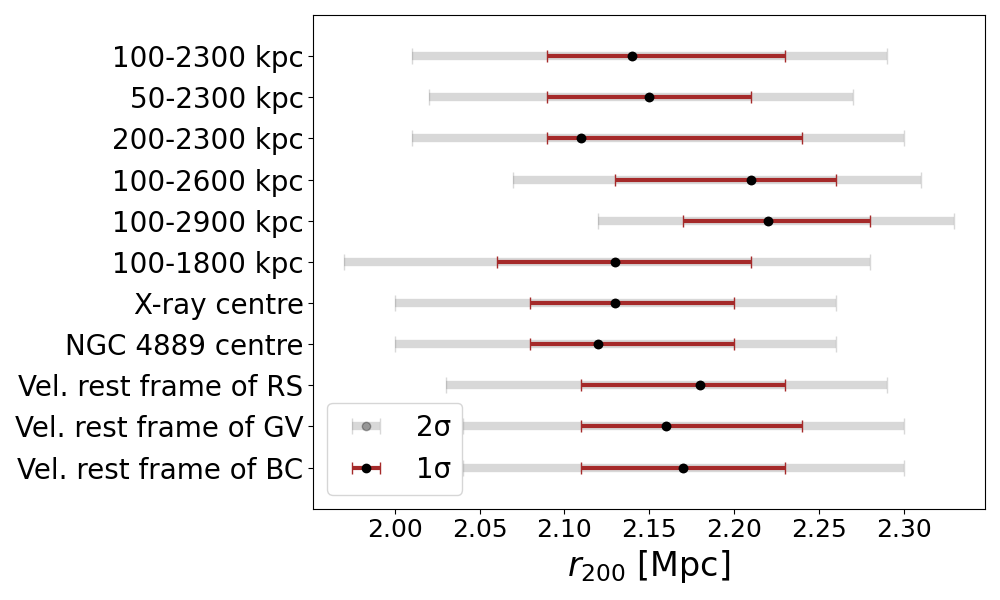
\includegraphics[width=0.5\linewidth]{images/r200_intervals.png}
    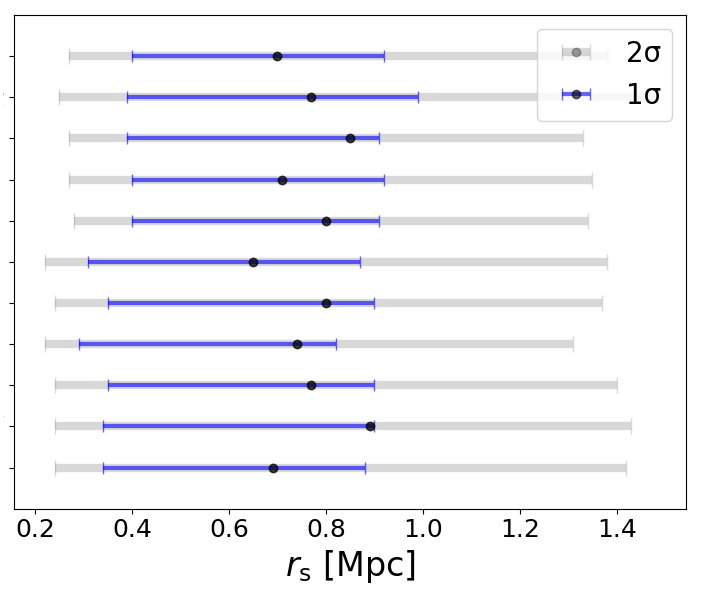
\includegraphics[width=0.35\linewidth]{images/rs_intervals.png}
    \caption{$r_{200}$ (left) and $r_{\text{s}}$ (right) estimates and confidence intervals ($1$ and $2\,\sigma$) for the different runs, specified on the left, performed to check the robustness of the mass modelling.}
    \label{fig:r200-rs-comparison}
\end{figure*} 


\begin{figure}
    \centering
    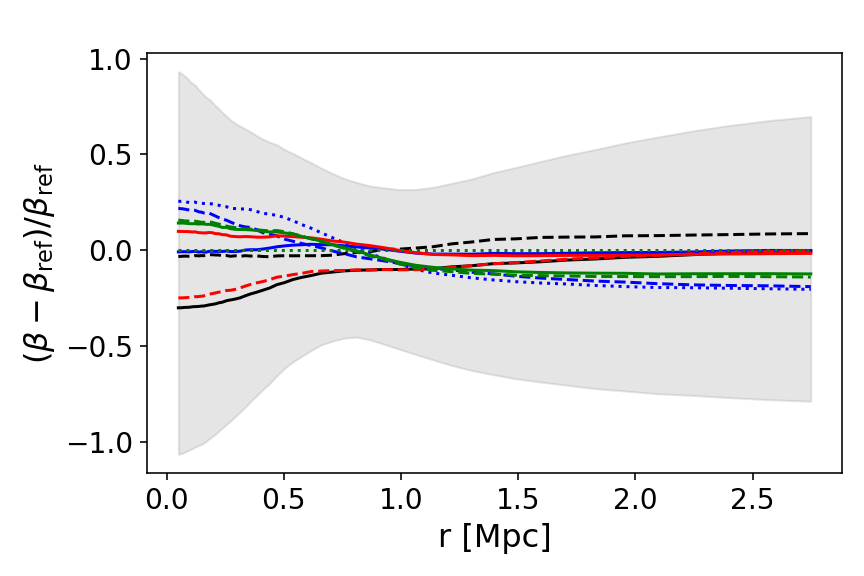
\includegraphics[width=0.9\linewidth]{images/relative_anisotropy.png}
    \caption{Relative variation of the anisotropy profiles with respect to the reference profile ($\beta_{\text{ref}}$) of Fig.~\ref{fig:anis_profile} after: changing minimum radius (black) to 50 kpc (solid) and 200 kpc (dashed); changing maximum radius (blue) to 1.8 Mpc (solid), 2.6 Mpc (dashed) and 2.9 Mpc (dotted); moving the cluster centre (red) to the coordinates of NGC 4889 (solid) and of the X-ray peak (dashed); shifting the velocity rest frame (green) to that of RS (solid), BC (dashed) and GV (dotted) galaxies. The grey band identifies the $1\,\sigma$ uncertainty band of the reference profile.       }
    \label{fig:relative_anis}
\end{figure} 

\subsection{Orbital anisotropy study for different colour classes}
\label{subsec:diff_sample_mamposst}


We devote this Section to the comparison of the anisotropy profiles of RS, GV, and BC galaxies. In fact, even if the profile obtained with the mixed sample does not show significant trends with radius (Fig.~\ref{fig:anis_profile}), it might be that different populations contribute differently to the orbital properties of the cluster. 

In general, given the evolutionary picture of galaxies in clusters described in Sect. \ref{sec:intro}, we would expect to observe a higher value of the anisotropy for BC and GV with respect to RS galaxies. However, the runs performed in Sect. \ref{full_sample_mamposst} for the different colour classes cannot be used to directly compare the anisotropy profiles, because the corresponding mass parameters are significantly different. While the values of $r_{\rm s}$ obtained from the different tracers are mutually consistent (note that the BC estimate presents very high uncertainties), this is not the case for $r_{200}$, for which the GV estimate is lower and the BC one is higher than that of the RS. This BC result supports the hypothesis proposed in Sect. \ref{subsec:LoS_methods}, namely that a substantial fraction of BC galaxies belongs to a filamentary-like structure along the LoS, leading to an overestimation of the cluster's virial radius. In order to directly compare the anisotropy profiles of the populations, we need their mass parameters to be consistent a priori; therefore, we performed additional \textsc{MG-MAMPOSSt} runs employing Gaussian priors on $r_{200}$ and $r_{\rm s}$ coming from the joint likelihood estimates of Sect. \ref{full_sample_mamposst}, obtained combining the RS, GV, and BC runs. The corresponding new results for all parameters and populations are reported in Table \ref{tab:diff_samples_results_withpriors}.
%--------------------------------------------------------
\begin{table}
\centering
\caption{Same as Table \ref{tab:diff_samples_results}, but for the runs with Gaussian priors on $r_{200}$ and $r_{\rm{s}}$ from the joint likelihood.}
\renewcommand{\arraystretch}{1.3}
\begin{tabular}{lccc}
\hline
{Parameter} & {RS} & {GV} & {BC} \\
\hline
       
       $r_{200} \, (\mathrm{Mpc})$ & $2.10_{-0.05}^{+0.04}$ & $2.08_{-0.03}^{+0.08}$ & $2.16_{-0.06}^{+0.05}$ \\
       $r_{\rm s} \, (\mathrm{Mpc})$ & $0.58_{-0.25}^{+0.03}$ & $0.57_{-0.32}^{+0.06}$ & $0.74_{-0.28}^{+0.06}$ \\
       $r_\nu^{\rm H} \, (\mathrm{Mpc})$ & $1.27_{-0.08}^{+0.10}$ & $7.78_{-3.48}^{+0.75}$ & $6.62_{-1.52}^{+1.76}$ \\
       $\mathcal{A}_0$ & 
       $1.20_{-0.46}^{+0.47}$ & $1.76_{-0.95}^{+1.71}$ & $1.37_{-0.40}^{+1.08}$ \\
       $\mathcal{A}_\infty$ & $1.50_{-0.40}^{+0.07}$ & $1.24_{-0.38}^{+0.40}$ & $1.62_{-0.40}^{+0.60}$ \\
          
\hline
\end{tabular}
\caption*{\footnotesize \textbf{Notes.} Gaussian priors on $r_\nu^{\rm H}$ are based on the estimates of Sect. \ref{num_density_methods}, while those for $\mathcal{A}_0$ and $\mathcal{A}_\infty$ are flat (same as Table \ref{tab:priors_flat}).}
\label{tab:diff_samples_results_withpriors}
\end{table}
%--------------------------------------------------------


The obtained anisotropy profiles of the different populations are shown for RS, GV, and BC galaxies in Fig.~\ref{fig:anis_subsamples}. By also comparing these plots with Fig.~\ref{fig:anis_profile}, relative to the profile obtained with the mixed sample, we note that all the profiles are similar within the uncertainties, with broader 1 and $2\,\sigma$ regions in the centre (within $R \lesssim 1.0 \, \mathrm{Mpc}$) with respect to the outskirts. However, some differences in the median profiles are observed: in particular, the behaviour of RS galaxies is very similar to that of the mixed sample, showing a general tendency towards radial orbits both in the central regions and in the outskirts. BC galaxies, on the other hand, display even more radial orbits in the outskirts, while remaining similar to the RS population in the core. Finally, GV galaxies exhibit a strong increase in radial anisotropy in the central region, whereas their outer orbits remain comparable to those of RS galaxies. These results are consistent with a scenario in which young, star forming galaxies fall into the cluster from the outer regions and transition to the GV phase as they approach the cluster core, likely as a consequence of substantial ram-pressure stripping. This evolutionary pathway could be investigated splitting the sample in other subclasses (e.g. from the Star Formation Rate (SFR) vs $M_*$ diagram) but we do not expect significant differences in the results. As a simple test, we split the full sample of galaxies into two equal population stellar mass bins and performed the same \textsc{MG-MAMPOSSt} analysis as that for the three colour classes. The results are reported in Appendix \ref{app:high-vs-low-mass}. 

 %The tendency towards tangential orbits observed for young star forming galaxies may be driven by a selection effect: galaxies moving on radial orbits towards the cluster centre are more strongly affected by ram pressure stripping, which rapidly quenches their star formation, causing them to transition first to the GV and eventually to the RS. As a result, the blue galaxies observed in the cluster core today are preferentially those on tangential orbits, which are less affected by gas-stripping mechanisms. This naturally produces the anisotropy profile shown in Fig.~\ref{fig:anis_subsamples}.


%that the main differences rise in the core of the cluster (within $R \lesssim 0.5 \, \mathrm{Mpc}$), where the behaviour of RS galaxies is similar to that of the full sample, while those of BC and GV galaxies indicate a trend of departure from isotropy and a much more relevant radial component, especially for BC galaxies. %In the cases of GV and BC galaxies, only the $1\,\sigma$ interval is shown; this is because the $2\,\sigma$ regions are very broad and not particularly informative, reflecting the intrinsic difficulty in constraining the orbital anisotropy with a small number of galaxies in the subsamples.

\begin{figure*}
    \centering
    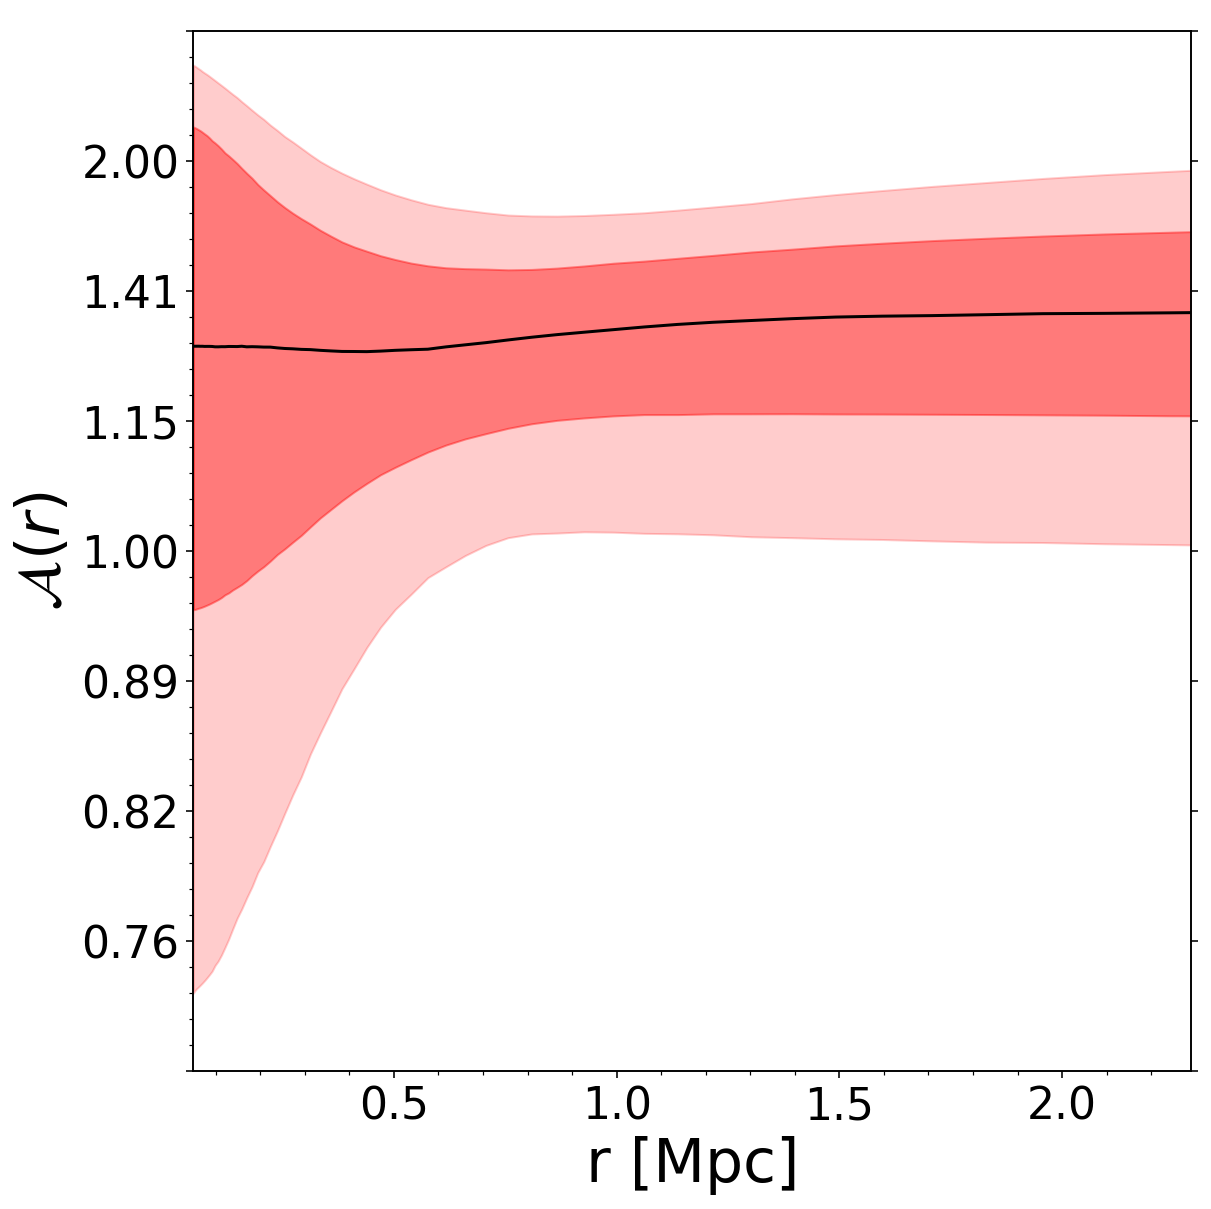
\includegraphics[width=0.2817\linewidth]{images/mamposst/diff_samples/anis_rosse.png}
    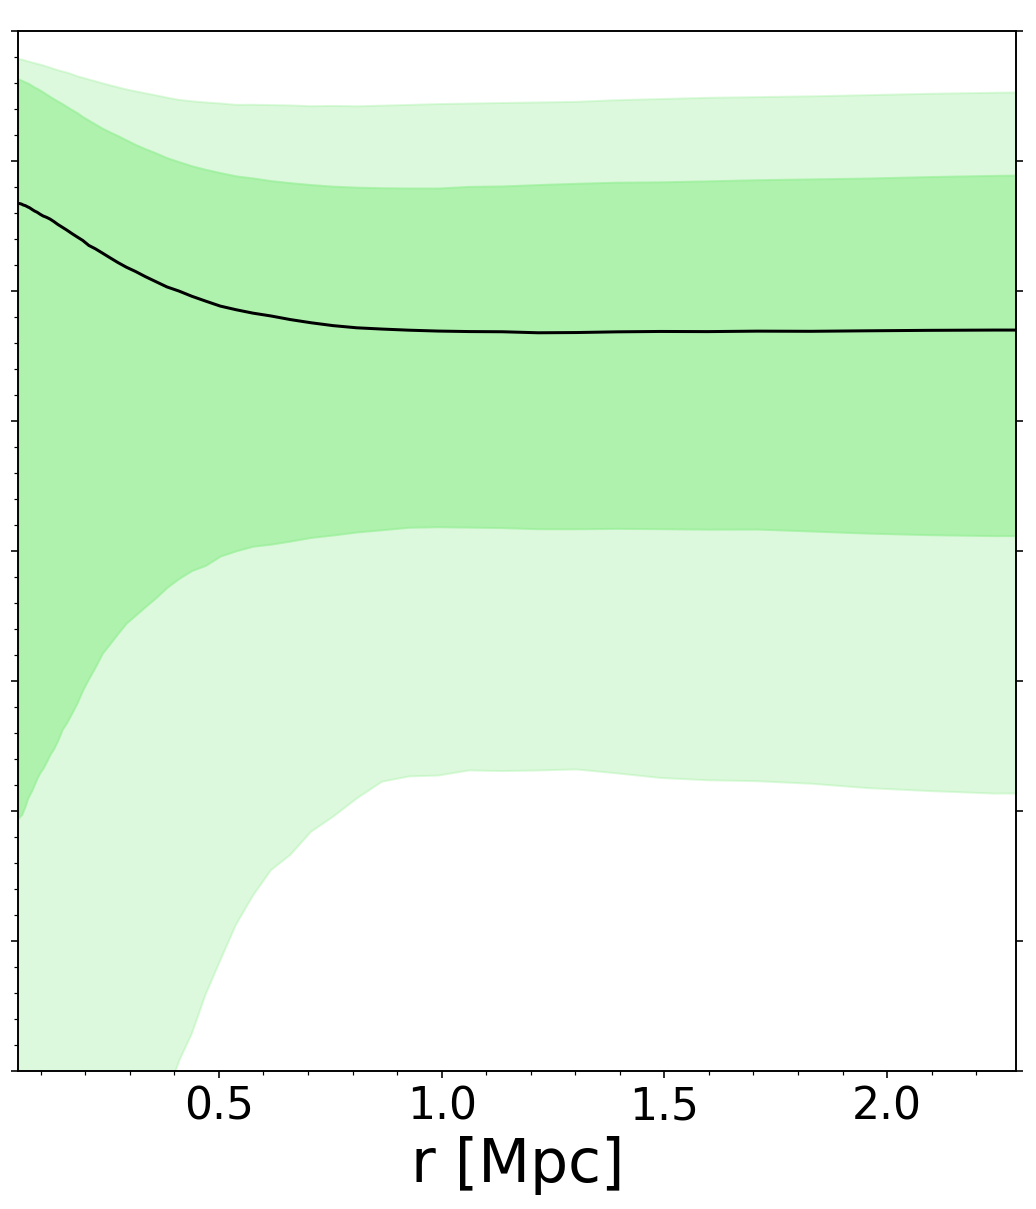
\includegraphics[width=0.241\linewidth]{images/mamposst/diff_samples/anis_verdi.png}
    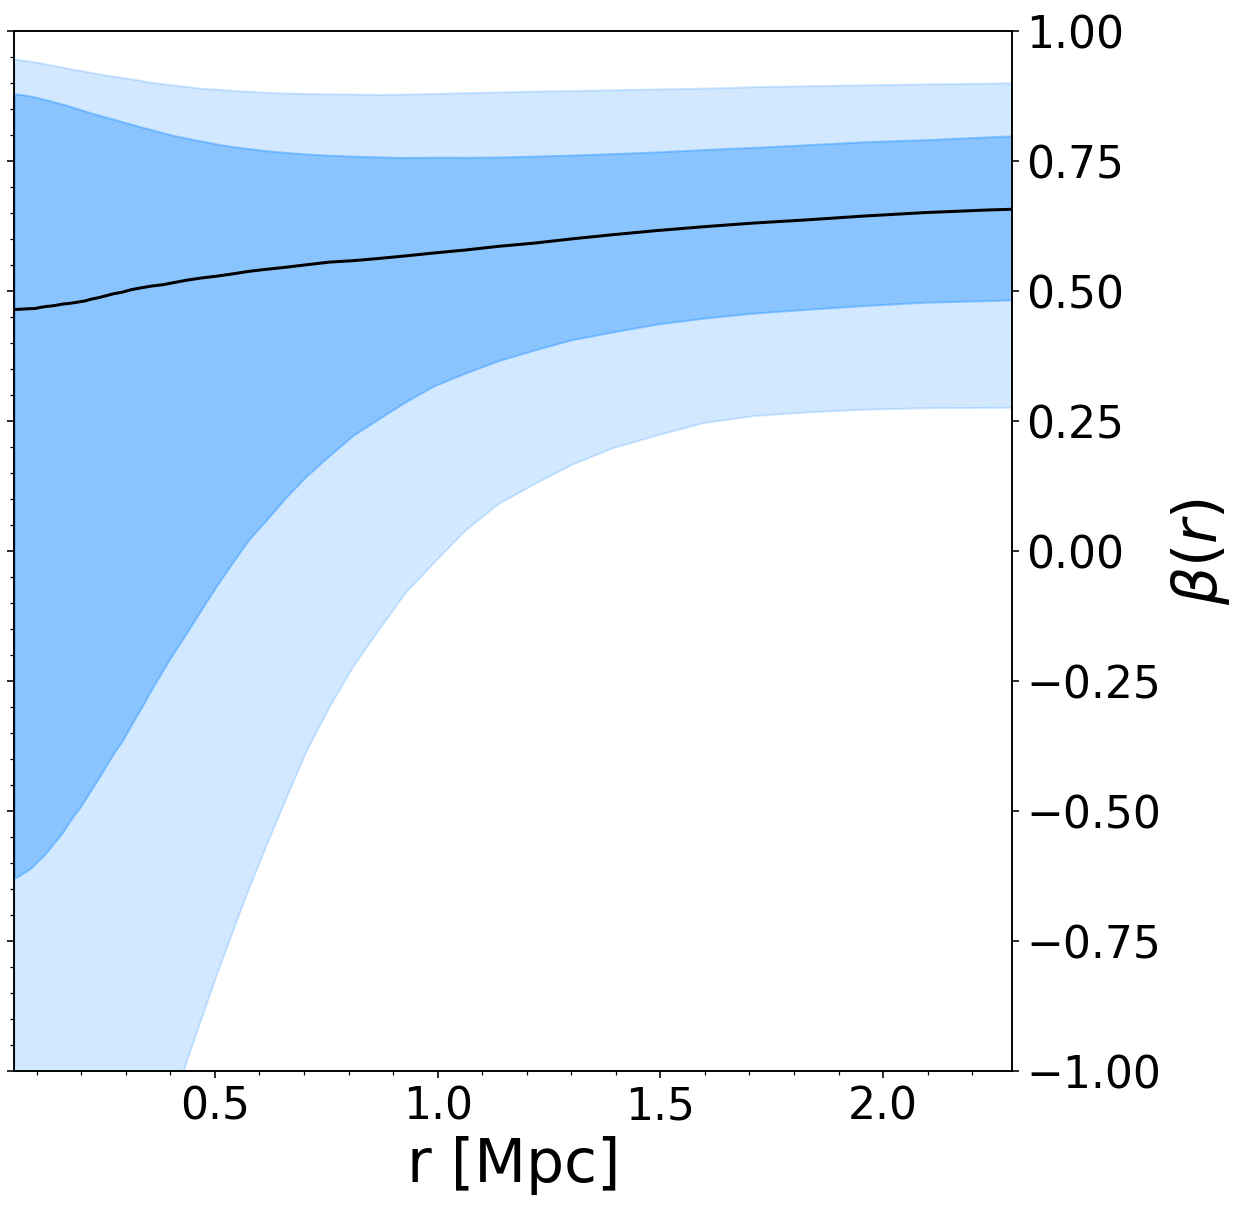
\includegraphics[width=0.29\linewidth]{images/mamposst/diff_samples/anis_blu.png}
    \caption{Estimated anisotropy profiles in NFW gOM runs with Gaussian priors on the mass (coming from the joint results of Sect. \ref{full_sample_mamposst}) for RS (left), GV (middle), and BC (right) galaxies, separately. The coloured and shaded regions indicate 1$\,\sigma$ and 2$\,\sigma$ confidence intervals, respectively. Solid curves are the median profiles of each MCMC chain.}
    \label{fig:anis_subsamples}
\end{figure*} 



%\subsection{Analysis of substructures}
%\label{subsec:substructures}

%Different \textbf{studies} (\textit{e.g., }\citealt{Adami_2005a, Adami_2005b, Healy_2021}) pointed out the presence of many substructures within the Coma Cluster, with the notable example of a massive group located south west (SW), centered around NGC 4839. The presence of one or more substructures in our sample is also suggested by the skewness of the LoS velocity distribution for BC galaxies towards positive rest frame velocities. This might be possibly related to a dominant population of young and star forming galaxies in one or more of those substructures, infalling towards the central region from the near-side of the cluster \citep{Biviano+96,Colless_1996}.

%We performed here an independent study of the substructures within the virial radius by applying the DS+ method by \citet{Benavides_2023}. This method only requires the projected positions and LoS velocities of member galaxies, being the natural improvement and extension of the traditional method developed by \citet{Dressler_1988}. 

%The results of this analysis are shown in Fig.~\ref{fig:substruct_den_vel}, where the member galaxies within $R\lesssim 2.1 \, \mathrm{Mpc}$ are displayed and coloured according to their belonging to a specific substructure, with the brightest galaxies of the sample being highlighted in yellow. We find 7 different substructures, with the two largest ones (SW and NW of the centre) that are consistent with the results of previous studies of Coma Cluster substructures (\textit{e.g.} \citealt{Adami_2005a,Adami_2005b}). We report the total number of galaxies, the stellar mass, the average LoS velocity, its uncertainty and the average radius of each substructure in Table \ref{tab:substruct_properties}. The SW group (number 4 in Fig.~\ref{fig:substruct_den_vel}), which extends in the tail of NGC 4839, is well known in the literature; the displacement between the brightest galaxy of the group and the gas left behind by the group motion is an indication of the infall of the substructure towards the central region \citep{Neumann_2003}, probably after reaching its first apocenter \citep{Lyskova+19}. 

%Another interesting substructure is number 5, NW of the centre, found around NGC 4841; this could be the remnant of the group dominated by NGC 4874 which impacted the cluster moving towards north. The major galaxy, due to its higher mass, could have been left behind and settled in the central region, together with NGC 4889, while the rest of group continued moving north. This scenario is supported by the observations of diffuse light by \citet{Adami_2005b} in the region north of NGC 4874, which typically comes from disrupted material or harassed galaxies, and by the presence of a bright X-ray emitting elongated area in the same region, possibly the shock front of the galaxy's motion \citep{Neumann_2003}. The same region is also characterized by a higher X-ray emitting gas temperature \citep{Churazov_2021}.
%The substructure number 1, directly west from the centre, could be the small overdensity group associated to NGC 4816. 

%\begin{figure}
 %   \centering
%    \includegraphics[width=1.2\linewidth]{images/DSp_xy_Coma_den_vel.pdf}
  %  \caption{Projected positions of member galaxies within $\lesssim 2.1 \, \mathrm{Mpc}$, shown as coloured squares when associated with a substructure (numbered from 1 to 7) and as empty white circles otherwise. The brightest galaxies are highlighted with filled yellow circles. The yellow dashed line marks the outer radial limit of 2.1 Mpc, while the solid yellow lines trace the iso-density contours of the projected galaxy number density, spaced at constant intervals of $\log_{10}$ of the density. In the background, the mean LoS velocity map ranges from $-800$ to $+600 \, \mathrm{km \, s^{-1}}$ (from dark to light).}
  %  \label{fig:substruct_den_vel}
%\end{figure} 

%We check the colours of the galaxies inside substructures, particularly looking for BC galaxies - for which the LoS veocity distribution deviates from Gaussianity. It turns out that, out of the 140 BC galaxies in our sample within the upper radius of the substructures analysis, only 27 reside in those overdensities (see Table \ref{tab:substruct} for the statistics). The LoS velocity distribution for the 113 BC galaxies within $\lesssim 2.1 \, \mathrm{Mpc}$ that are not found in substructures is shown in the top panel of Fig.~\ref{fig:blu_stat_subs}: evidently, the departure of the distribution from Gaussianity is not solved by removing galaxies in substructures, which is confirmed by the resulting Anderson-Darling coefficient of $A^2\sim1.61$, similar to that of the overall BC distribution (Fig.~\ref{fig:vel_LoS}). We also show, at the bottom of the same Figure, the LoS velocity distribution for the 109 BC galaxies with $R \gtrsim 2.1 \, \mathrm{Mpc}$, for which we do not have information on sub-clustering. In this case, the deviations from Gaussianity are mitigated with respect to the general case, with a coefficient $A^2=0.99$. This indicates that the main sources of the observed LoS velocity deviations towards positive values are galaxies that reside within the virial region in projected space. 

%\begin{table}
%\caption{Properties of the 7 small-scale substructures of Coma.}
%\centering
%\renewcommand{\arraystretch}{1.3}
%\resizebox{\columnwidth}{!}{
%\begin{tabular}{l c c S c}
%\hline
%{Substructure} & {N} & { $M_*$} & { $\langle v_\text{RF} \rangle $}  & { $\langle R \rangle$} \\
%{} & {} & {[$10^{11} \, M_\odot$]} & {[$\mathrm{km/s}$]} & {[$\mathrm{Mpc}$]} \\

%\hline
%1   & 20   & 5.13  & -123 \pm 11   & 0.110  \\
%2   & 20   & 0.51  & -666 \pm 11  & 0.320 \\
%3   & 20   & 1.14  & 536 \pm 11 & 0.175 \\
%4   & 79   & 9.27  & 407 \pm 6   & 0.349  \\
%5   & 80   & 8.66  & 103 \pm 6  & 0.362 \\
%6   & 20   & 3.20  & -628 \pm 11   & 0.132 \\
%7   & 20   & 1.16  & 720 \pm 11   & 0.081 \\
%\hline
%\end{tabular}
%\caption*{\footnotesize \textbf{Notes.} The columns represent, in order: the substructure ID in Fig.~\ref{fig:substruct_den_vel}, the total number of galaxies, the total stellar mass, the average recessional velocity in the cluster's rest frame with its uncertainty and the average radius of the substructure. }
%\label{tab:substruct_properties}
%\end{table}



%\begin{table}
%\centering
%\caption{Statistic relative to the colour of galaxies in each substructure.}
%\renewcommand{\arraystretch}{1.3}
%\resizebox{\columnwidth}{!}{
%\begin{tabular}{l 
                %S[table-format=3.0] 
                %S[table-format=3.0] 
                %S[table-format=3.0] 
                %S[table-format=2.1] 
                %S[table-format=2.1] 
                %S[table-format=2.1]}
%\hline
%{Substructure} & {RS} & {GV} & {BC} & { $P_{\rm RS}\%$} & { $P_{\rm GV}\%$} & { $P_{\rm BC}\%$} \\
%\hline
%None & 818 & 100 & 113 & 79.3 & 9.7 & 11.0 \\
%1    & 16  & 1  & 0   & 94.1 & 5.9 & 0.0  \\
%2    & 14  & 3  & 3   & 70.0 & 15.0 & 15.0 \\
%3    & 12  & 2  & 4   & 66.7 & 11.1 & 22.2 \\
%4   & 70  & 2  & 3   & 93.3 & 2.7 & 4.0  \\
%5    & 58  & 6  & 13  & 75.3 & 7.8 & 16.9 \\
%6    & 10  & 7  & 1   & 55.6 & 38.9 & 5.6 \\
%7    & 17  & 0  & 3   & 85.0 & 0.0 & 15.0 \\
%\hline
%\end{tabular}}
%\caption*{\footnotesize \textbf{Notes.} The columns represent, in order: the substructure ID in Fig.~\ref{fig:substruct_den_vel}, the number of RS, GV and BC galaxies and the relative percentages. Galaxies excluded from the colour classification are not considered in this table.}
%\label{tab:substruct}
%\end{table}



%\begin{figure}
 %   \centering
 %   \includegraphics[width=0.65\linewidth]{images/blu_vel_outside_substr.png}
 %   \includegraphics[width=0.65\linewidth]{images/blu_vel_outside_vir.png}
 %   \caption{LoS velocity distributions of blue cloud galaxies within $R \lesssim 2.1 \, \mathrm{Mpc}$ and outside the identified substructures (top) and of blue cloud galaxies outside the projected region $R \sim2.1 \, \mathrm{Mpc}$ (bottom). The vertical dashed line marks the rest frame of the cluster. }
  %  \label{fig:blu_stat_subs}
%\end{figure}

%Finally, we aimed at assessing the robustness of our kinematic mass estimate by running \textsc{MG-MAMPOSSt} on the full sample of galaxies within $R \lesssim 2.1 \,\mathrm{Mpc}$ but excluding those in substrutures identified by DS+. The resulting mass profile is in excellent agreement with our reference analysis (Sect.~\ref{full_sample_mamposst}), with a virial mass $M_{200} = 1.10_{-0.13}^{+0.12} \times 10^{15} \, M_\odot$.

%\subsection{Cosmological simulation}

%\begin{figure}
 %   \centering
    %\includegraphics[width=.9\linewidth]{images/Filament_SimulationMarks.png}
    %\caption{}
    %\label{}
%\end{figure}

%The BC galaxies that are responsible for the LoS velocity distribution distortion lie in the projected virial region of Coma but are not sufficiently clustered together to be identified by DS+ as members of a substructure. 
%This picture points to the possible presence of a filamentary-like structure at the near side of the cluster along the LoS, from which BC galaxies are infalling towards the cluster.

%In order to verify if such a scenario would be consistent with our results, we consider a single snapshot taken from a $\Lambda$CDM N-body hydrodynamic cosmological simulations presented in \cite{Ragagnin_2024}, run with the Gadget~\citep{Springel2005} code, using initial conditions from DIANOGA zoom-in simulations~\citep{Bonafede2011,Rasia2015,Ragone-Figueroa2018}, re-simulated with Magneticum physics~\citep[e.g.,][]{Tornatore2004,Hirschmann2014,Dolag2025}.

%We focus on a massive halo of total mass $M \sim 10^{15} \,M_\odot$ at low redshift, identifying a filamentary-like structure linked to the halo; we performed a rotation to align the filament with the LoS (circled in Fig.~\ref{fig:halo_1}). At this point we consider a sample of $5000$ particles belonging to the filament with a displacement from the cluster centre of more than $r_{200}$, and we compare their LoS velocity distribution with that of particles with $|z|<r_{200}$ in the virial projected region. The resulting distributions are shown in Fig.~\ref{fig:halo_2}, as well as the positions of galaxies in the projected plane; the LoS velocity distribution of filament galaxies indeed exhibits a deviation towards positive rest frame velocities, peaking at $1000$ km/s, while the rest of the sample shows a much more relaxed behavior. This is consistent with the LoS velocity distribution obtained with the Coma Cluster member galaxies belonging to the BC subsample, making the hypothesis of a filamentary-like structure along the LoS our best guess in explaining their unrelaxed distribution.  

%\begin{figure}
  %  \centering
  %  \includegraphics[width=.7\linewidth]{images/Filament_SimulationMarks2.png}
  %  \caption{2D distribution of galaxies in the massive halo from the cosmological simulation. The circled filamentary like structure is aligned with the LoS, considered as the $z$ direction. }
   % \label{fig:halo_1}
%\end{figure}


%\begin{figure}
  %  \centering
  %  \includegraphics[width=.7\linewidth]{images/Filament_SimulationMarks4.png}
  %  \includegraphics[width=.7\linewidth]{images/Filament_SimulationMarks3.png}
  %  \caption{Top panel: projected 2D distribution ($x$ and $y$ in kpc) of galaxies in the virial region of the massive halo from the cosmological simulation. In red are all galaxies with $|z|<r_{200}$ and in blue those belonging to the filament along the LoS with $z<-r_{200}$. Bottom panel: Normalized LoS velocity distributions for the two corresponding samples.}
   % \label{fig:halo_2}
%\end{figure}


%\subsection{Mass--concentration relation}

%We also test the observed concentration ($c_{200} = 3.9^{+1.8}_{-1.1}$, from the results of Sect.~\ref{full_sample_mamposst}) with theoretical studies in the literature. These works show that concentration estimates can be biased towards higher values if clusters are older~\citep[][and therefore gas-poor]{Ragagnin2022} or due to LoS elongation and the presence of filaments \citep{Meneghetti2014,Giocoli2024,Ragagnin2025}. Since massive clusters are rarely highly relaxed or gas-poor, we expect the Coma cluster to exhibit a larger-than-average concentration as a consequence of its alignment along the LoS. To this end, we estimate the average concentration for a $10^{15}\,{\rm M_\odot}$ galaxy cluster using the multi-cosmology Magneticum simulations~\citep{Singh2020} and the mass--concentration fits presented in~\cite{Ragagnin2021}\footnote{\url{https://c2papcosmosim.uc.lrz.de/static/hydro_mc/webapp/index.html}}, obtaining $c_{200}=3.4,$ that is only slightly lower than the value from our best fit value, and well between the 68\% confidence limit. It is important to stress that a previous kinematical estimate of the Coma cluster concentration from \cite{Lokas_2003} found a surprisingly large value of $c_{200}\sim 7$, while the analysis of \cite{Gavazzi_2009} found a value $5^{+3}_{-2}$, which is in agreement with our results. 

%On the other hand, the observational constraint on the concentration of the Coma cluster of this work is $c_{200}\simeq 3.9$ (see Sect.~\ref{full_sample_mamposst}, where $r_{200}=2.07\,{\rm Mpc}$ and $r_{\rm s}=0.53\,{\rm Mpc}$). This value is higher than the mean expected for this mass bin and cosmology and is consistent with an alignment along the LoS.





\section{Conclusions}
\label{sec:conclusions}
%The main purpose of this work is to investigate the fundamental connection between dynamical and morphological properties of galaxies in dense environments. In order to do so, we have focused our study to

In this work, we performed a detailed kinematic analysis of the Coma Cluster using a novel rich spectroscopic catalogue of cluster members from the DESI survey. We applied the \textsc{MG-MAMPOSSt} code to a sample of 1324 member galaxies in the projected phase space ($R, v_\text{RF}$) up to $R \sim 2.3$ Mpc, in order to jointly reconstruct the mass and orbital anisotropy profiles of Coma. By working with different subsamples of member galaxies, selected based on their colour, we obtained useful insights about the effect of the internal cluster dynamics on the properties of member galaxies.

\begin{figure}
    \centering
    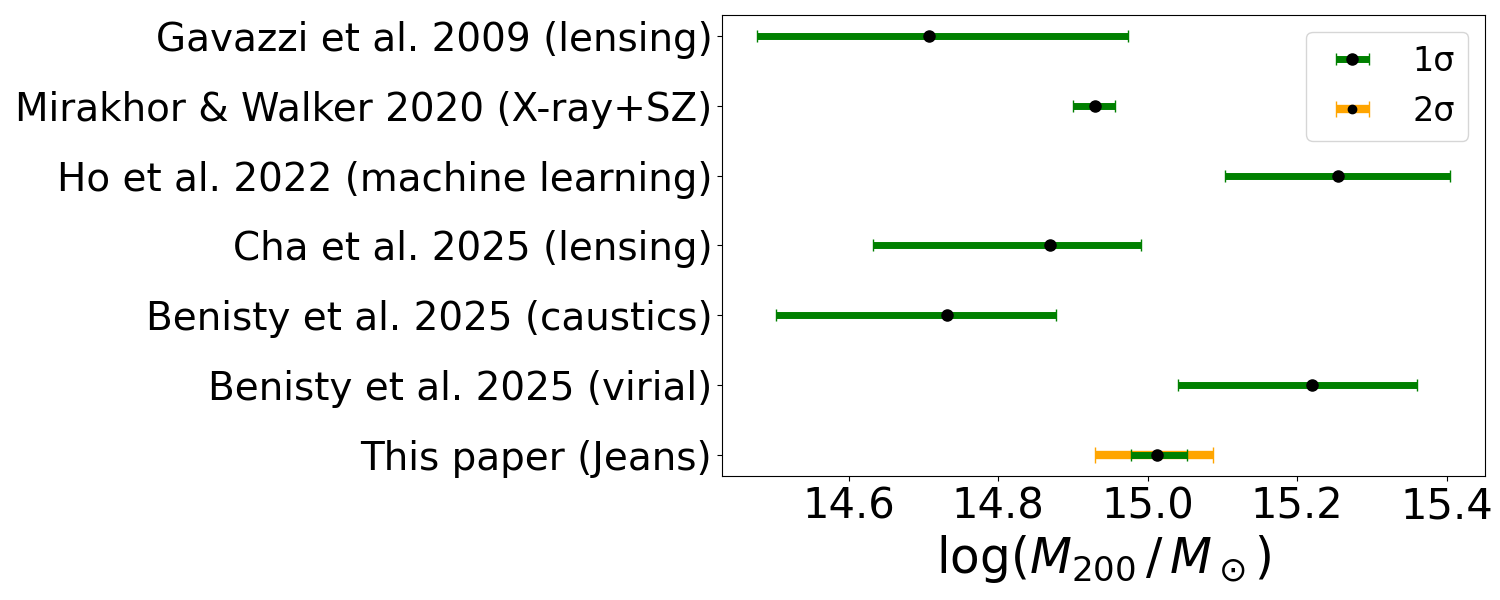
\includegraphics[width=0.9\linewidth]{images/mass_comparison_papers.png}
    \caption{Comparison between $M_{200}$ estimates from different studies (indicated on the left of the figure) and our best estimate from \textsc{MG-MAMPOSSt} with DESI dataset.}
    \label{fig:mass_compare}
\end{figure} 
We found that blue cloud (BC) galaxies, contrary to red sequence (RS) galaxies, exhibit strong deviations from Gaussianity in their LoS velocity distribution. This behaviour is consistent with theoretical predictions about LTGs still infalling towards the cluster centre, along more elongated orbits, in which the efficiency of ram-pressure stripping is higher in quenching star formation, thereby contributing to their eventual transition into ETGs. %We point out a prevalence of BC galaxies with positive LoS velocities in the rest frame of the cluster and residing in the virial region in projected space, a possible indication of a filamentary-like structure at the near-side of the cluster along the LoS; this interpretation is further supported by the analysis of snapshots from available cosmological simulations.

We ran \textsc{MG-MAMPOSSt} on the full sample of member galaxies and on different colour subsamples, exploring various combinations of mass and anisotropy models. While all the models provide adequate fits of the total mass distribution, the NFW profile  with gOM anisotropy gives the lowest BIC/AIC; we quote the Coma Cluster's virial mass, obtained from the joint likelihood of the different populations, to be $M_{200} = 1.08_{-0.09}^{+0.08}~({\rm stat}) \pm 0.09~({\rm syst}) \times 10^{15}  \, \mathrm{M_\odot}$, corresponding to $r_{200}=2.12 \pm 0.06~({\rm stat})\pm0.07~({\rm syst}) \, \mathrm{Mpc}$, where the systematic uncertainties account for the variation in the mode of the distribution among the combination of models and configurations tested, and the scale radius of the mass profile to be $r_{\rm s}=0.48_{-0.13}^{+0.27} \, \mathrm{Mpc}$. When separately including the gas and stellar mass in galaxies in the fit, we estimate a dark matter virial mass  $M_{200}^{\rm DM} = 8.6^{+1.2}_{-0.8}\times 10^{14}\, \,\text{M}_\odot$ and a baryon fraction $f_b = 0.15 \pm 0.02$ at $r = 2.12$ Mpc, in agreement with current cosmological studies.
%We have further estimated the impact of the dynamical state of the cluster on our constraints by running again \textsc{MG-MAMPOSSt} excluding galaxies in substructure, finding a negligible effect within statistical uncertainties.

Fig.~\ref{fig:mass_compare} shows a graphic comparison between our $M_{200}$ estimate and those from recent studies, in which different techniques have been adopted: weak lensing analysis, combination of X-ray and SZ effect, machine learning, caustics, and virial theorem methods. Interestingly, our best-fit value lies above the masses derived from lensing \citep{Gavazzi_2009, Cha_2025}, X-ray+SZ \citep{Mirakhor_2020} and caustics methods \citep{Benisty25} but below the ones inferred from machine-learning \citep{Ho_2022} and virial theorem methods \citep{Benisty25}. The $2\,\sigma$ error bars of our measurement overlap with $1\,\sigma$ error bars of lensing, X-ray+SZ, and virial theorem estimates, while approaching, but not reaching, the $1\,\sigma$ error bars from machine learning and caustics.

The anisotropy profile shows a tendency to radial orbits both in the centre and in the outskirts, similarly to the profile obtained by \citet{Pizzuti_2025b} for the cluster PSZ2 G067.17+67.46. %for stacked CHEX-MATE clusters at $z<0.4$.
The average $\beta(r)$ found by \citet{Biviano25} analysing nine massive clusters from the CLASH-VLT dataset shows a similar trend, with a slightly more isotropic behaviour in the centre, as well as the orbits found for ram pressure stripped member galaxies in nearby clusters \citep{Biviano24}. The parameter's behaviour remains comparable between RS, GV, and BC galaxies; however, the median profiles of GV and BC galaxies show even more substantial radial tendencies in the centre and in the outskirts, respectively, while RS galaxies produce a similar profile to the mixed sample. These results are consistent with many previous anisotropy studies of different galaxy populations, which report no significant differences between the orbits of passive and star forming galaxies in clusters \citep[\textit{e.g.}][]{Hwang_2008, Biviano_2013}. %However, some indications of tangential bias for the orbits of star forming galaxies in the central regions of clusters can be found in the results of cosmological hydrodynamical simulations (see Fig.~3 in \citealt{Lotz_2019}), even if at larger $z$.
The more radial behaviour of blue galaxies in the outer regions with respect to the red ones is consistent with the outcome of \citet{Mamon_2019} analyses (see \textit{e.g.} Fig.~7) of stacked clusters from WINGS. 
Also, our virial mass estimates significantly differ depending on the employed tracers, with BC galaxies producing a quite larger value; this may be an indication of a filamentary-like structure along the LoS, which we will deeply investigate in the upcoming paper II. The new study will focus on the substructure content of the Coma Cluster, the possibility of a recent major merging (see \citealt{Biviano+96}) and the implication of the dynamical state in the mass-orbit modelling.

%Lastly, we performed a substructure analysis of the Coma Cluster using the DS+ code \citep{Benavides_2023} finding 7 different substructures (Figure \ref{fig:substruct_den_vel}), with the two largest ones (SW and NW of the centre) that are consistent with the results of previous studies of Coma Cluster substructures \citep{Adami_2005a, Adami_2005b}. We confirm that the BC galaxies in these substructures are not the main source of the deviation of their LoS velocity distribution.

In summary, this work provides an important example of how studying galaxy clusters properties through a kinematic approach is a very useful strategy to constrain different scenarios of galaxy evolution. With the advent of new wide-field spectroscopic surveys, providing larger and more complete samples of galaxies in clusters, this approach will allow increasingly detailed and statistically robust studies of cluster dynamics and galaxy accretion, thereby offering new insights into the role of environment in shaping galaxy properties.


\begin{acknowledgements}
LP acknowledges support by the Italian Ministry for Research and University (MUR) under 457 Grant ``Progetto Dipartimenti di Eccellenza 2023-2027'' (BiCoQ).
LP and AR acknowledge the usage of INAF-OATs IT framework~\citep{Taffoni2020,Bertocco2020}.
AR acknowledges EuroHPC Joint Undertaking for awarding the project ID EHPC-REG-2024R01-029  access to Leonardo at CINECA, Italy.
AR acknowledges ISCRA for awarding this project access to the LEONARDO supercomputer, owned by the EuroHPC Joint Undertaking, hosted by CINECA, Italy (HP10BUFI59).
\end{acknowledgements}

\clearpage

\bibliographystyle{aa} % style aa.bst
\bibliography{biblio}

\appendix
\section{Impact of the assumed number density model}
\label{app:A}

For all the \textsc{MG-MAMPOSSt} runs discussed in the previous sections, we assumed a projected Hernquist model for the number density of member galaxies, with its scale radius $r_\nu$ (we drop the superscript 'H' in this Appendix, since it is always clear what model we are using) kept as a free parameter with flat informative priors based on our preliminary fits of Sect.~\ref{num_density_methods}. 

%However, this can introduce systematic biases in both the mass and anisotropy profiles.
Here we want to check, using \textsc{MG-MAMPOSSt}, that:
\begin{enumerate}
    \item[\textit{i)}] The projected Hernquist model is actually favoured by the \textsc{MG-MAMPOSSt} likelihood with respect to the NFW model.
    \item[\textit{ii)}] Even if $r_\nu$ is a free parameter, its best estimate is consistent with our first estimate of Sect.~\ref{num_density_methods}.
    \item[\textit{iii)}] The model with $r_\nu$ fixed at our best fit of Sect.~\ref{num_density_methods} is not favoured with respect to the case in which it is a free parameter.
\end{enumerate}

\noindent Table \ref{tab:model_comparison} shows the details of the runs performed, with relative priors and outcomes, to check \textit{i)--iii)}. The first two rows illustrate the comparison between projected NFW and projected Hernquist models: in these runs, $r_\nu$ is a free parameter, together with $r_{200}$, $r_{\rm s}$, $\mathcal{A}_0$ and $\mathcal{A_\infty}$. For $r_\nu$ we assume informative flat priors coming from our best fit estimate of Sect.~\ref{num_density_methods}, for $r_{200}$ and $r_{\rm s}$ we use broad and flat priors, as well as for the anisotropy parameters (same as Table \ref{tab:priors_flat}). We use the BIC and AIC criteria (Eq. \ref{eq:BIC} and \ref{eq:AIC}), already used in Sect.~\ref{full_sample_mamposst}, to evaluate the relative performance of the models. Both BIC and AIC favour the Hernquist model with respect to the NFW model: %this is surprising, considering that, for example, \citet{Mamon_2019} find that the Bayesian evidence rejects the Hernquist model compared to the NFW model. Nonetheless, 
we have tested this conclusion with several runs on different samples, including the three colour classes, and mass/anisotropy models, reaching the same outcome. This validates our first assumption and excludes any systematic errors caused by the employed numerical density model.

Also our second assumption is verified by the first two rows of Table \ref{tab:model_comparison}: in fact, the best fit estimates of $r_\nu$ from \textsc{MG-MAMPOSSt} are consistent with the fits performed in Sect.~\ref{num_density_methods}. Using the NFW model, the two estimates are almost exactly the same, while for the Hernquist model the best fit value is lower, but well within the $1\,\sigma$ interval. 

The results of the third and fourth row show what happens if we treat $r_\nu$ as a fixed input parameter. In these runs, the flat priors for $r_\nu$ are very tight around the best fit value from Sect. \ref{num_density_methods}; in practice, we mimic a fixed tracer scale radius by adopting a very narrow flat prior for $r_\nu$ and
reduce by hand the number of free parameters by unity. The reason why we do not consider $r_\nu$ as an actual fixed input parameter is that \textsc{MG-MAMPOSSt} uses a different expression for the fit depending on whether $r_\nu$ is a fixed or free parameter \citep{Mamon_2013}, invalidating the comparison of the likelihoods between the two cases. 
The results show that keeping $r_\nu$ 'fixed' with the NFW model produces an improvement of 7 BIC and 2 AIC units with respect to the free parameter case, while with the Hernquist model the BIC is improved by 4 but the AIC worsens by 2 units. Since the two criteria give conflicting indications for the adopted (Hernquist) model, we chose to treat $r_\nu^{\rm H}$ as a free parameter, which we consider the safest strategy. 


\begin{table*}
\centering
\caption{MG-MAMPOSSt priors and results for changes on tracer numerical density models.}
\renewcommand{\arraystretch}{1.3} % <-- più spazio tra righe
%\resizebox{\columnwidth}{!}{%
\begin{tabular}{lccccccc}
\hline
{Model} & {Min}\,$r_\nu \, (\mathrm{Mpc})$ & {Max}\,${r_\nu \, (\mathrm{Mpc})}$ & {Best fit} ${r_\nu \, (\mathrm{Mpc})}$ & ${k}$ & ${-\log\mathcal{L}}$ & {BIC} & {AIC} \\
\hline
NFW  & 0.59 & 0.86 & $0.70^{+0.05}_{-0.06}$  & 5 & 12\,209.84  & 24\,455 & 24\,429 \\
Hernquist  & 1.41 & 2.05 & $1.73^{+0.06}_{-0.16}$  & 5 & 12\,207.59  & 24\,451 & 24\,425 \\
NFW   & 0.709 & 0.711  & $0.71$  & 4 & 12\,209.78  & 24\,448 & 24\,427 \\
Hernquist & 1.929 & 1.931 & 1.93 & 4 & 12\,209.56 & 24\,447 & 24\,427 \\
\hline
\end{tabular}
\caption*{\footnotesize \textbf{Notes.} %Comparison of the relative performance of different models in fitting the data, to evaluate the validity of the assumptions made.
The columns report, in order, the employed model for the projected number density profile, the minimum and maximum limit of the flat employed priors, the best fit values for $r_\nu$, the number of free parameters $k$, the minimum value for the negative log-likelihood, the BIC and AIC parameters. The number of free parameters for the third and fourth rows was decreased by one to mimic a constant value for $r_\nu$.}
\label{tab:model_comparison}
\end{table*}



\section{Numerical profiles for different galaxy populations}
\label{app:B}

Fig.~\ref{fig:surface_density_subsamples} displays the projected surface density profiles of the different subsamples (RS, GV, BC) of galaxies, fitted with a projected Hernquist model. The low statistics of GV and BC samples are at the origin of the high uncertainties on the best fit scale radii (Sect.~\ref{num_density_methods}).

%\begin{figure}[!h]
 %   \centering
  %  \includegraphics[width=0.9\linewidth]{images/rscale_fit_RS.png}
  %  \includegraphics[width=0.9\linewidth]{images/rscale_fit_GV.png}
   % \includegraphics[width=0.9\linewidth]{images/rscale_fit_BC.png}
    %\caption{Numerical density profile of red sequence (top), green valley (middle) and blue cloud (bottom) galaxies in the Coma Cluster fitted with a pNFW model with, respectively, $r_\nu = 0.51 \, \text{Mpc}, 7.43 \,\text{Mpc} \,\text{and}\, 3.08 \, \text{Mpc}$. The error bars correspond to the Poisson uncertainties.}
   % \label{fig:num_density_subsamples}
%\end{figure} 

\begin{figure}[!h]
    \centering
    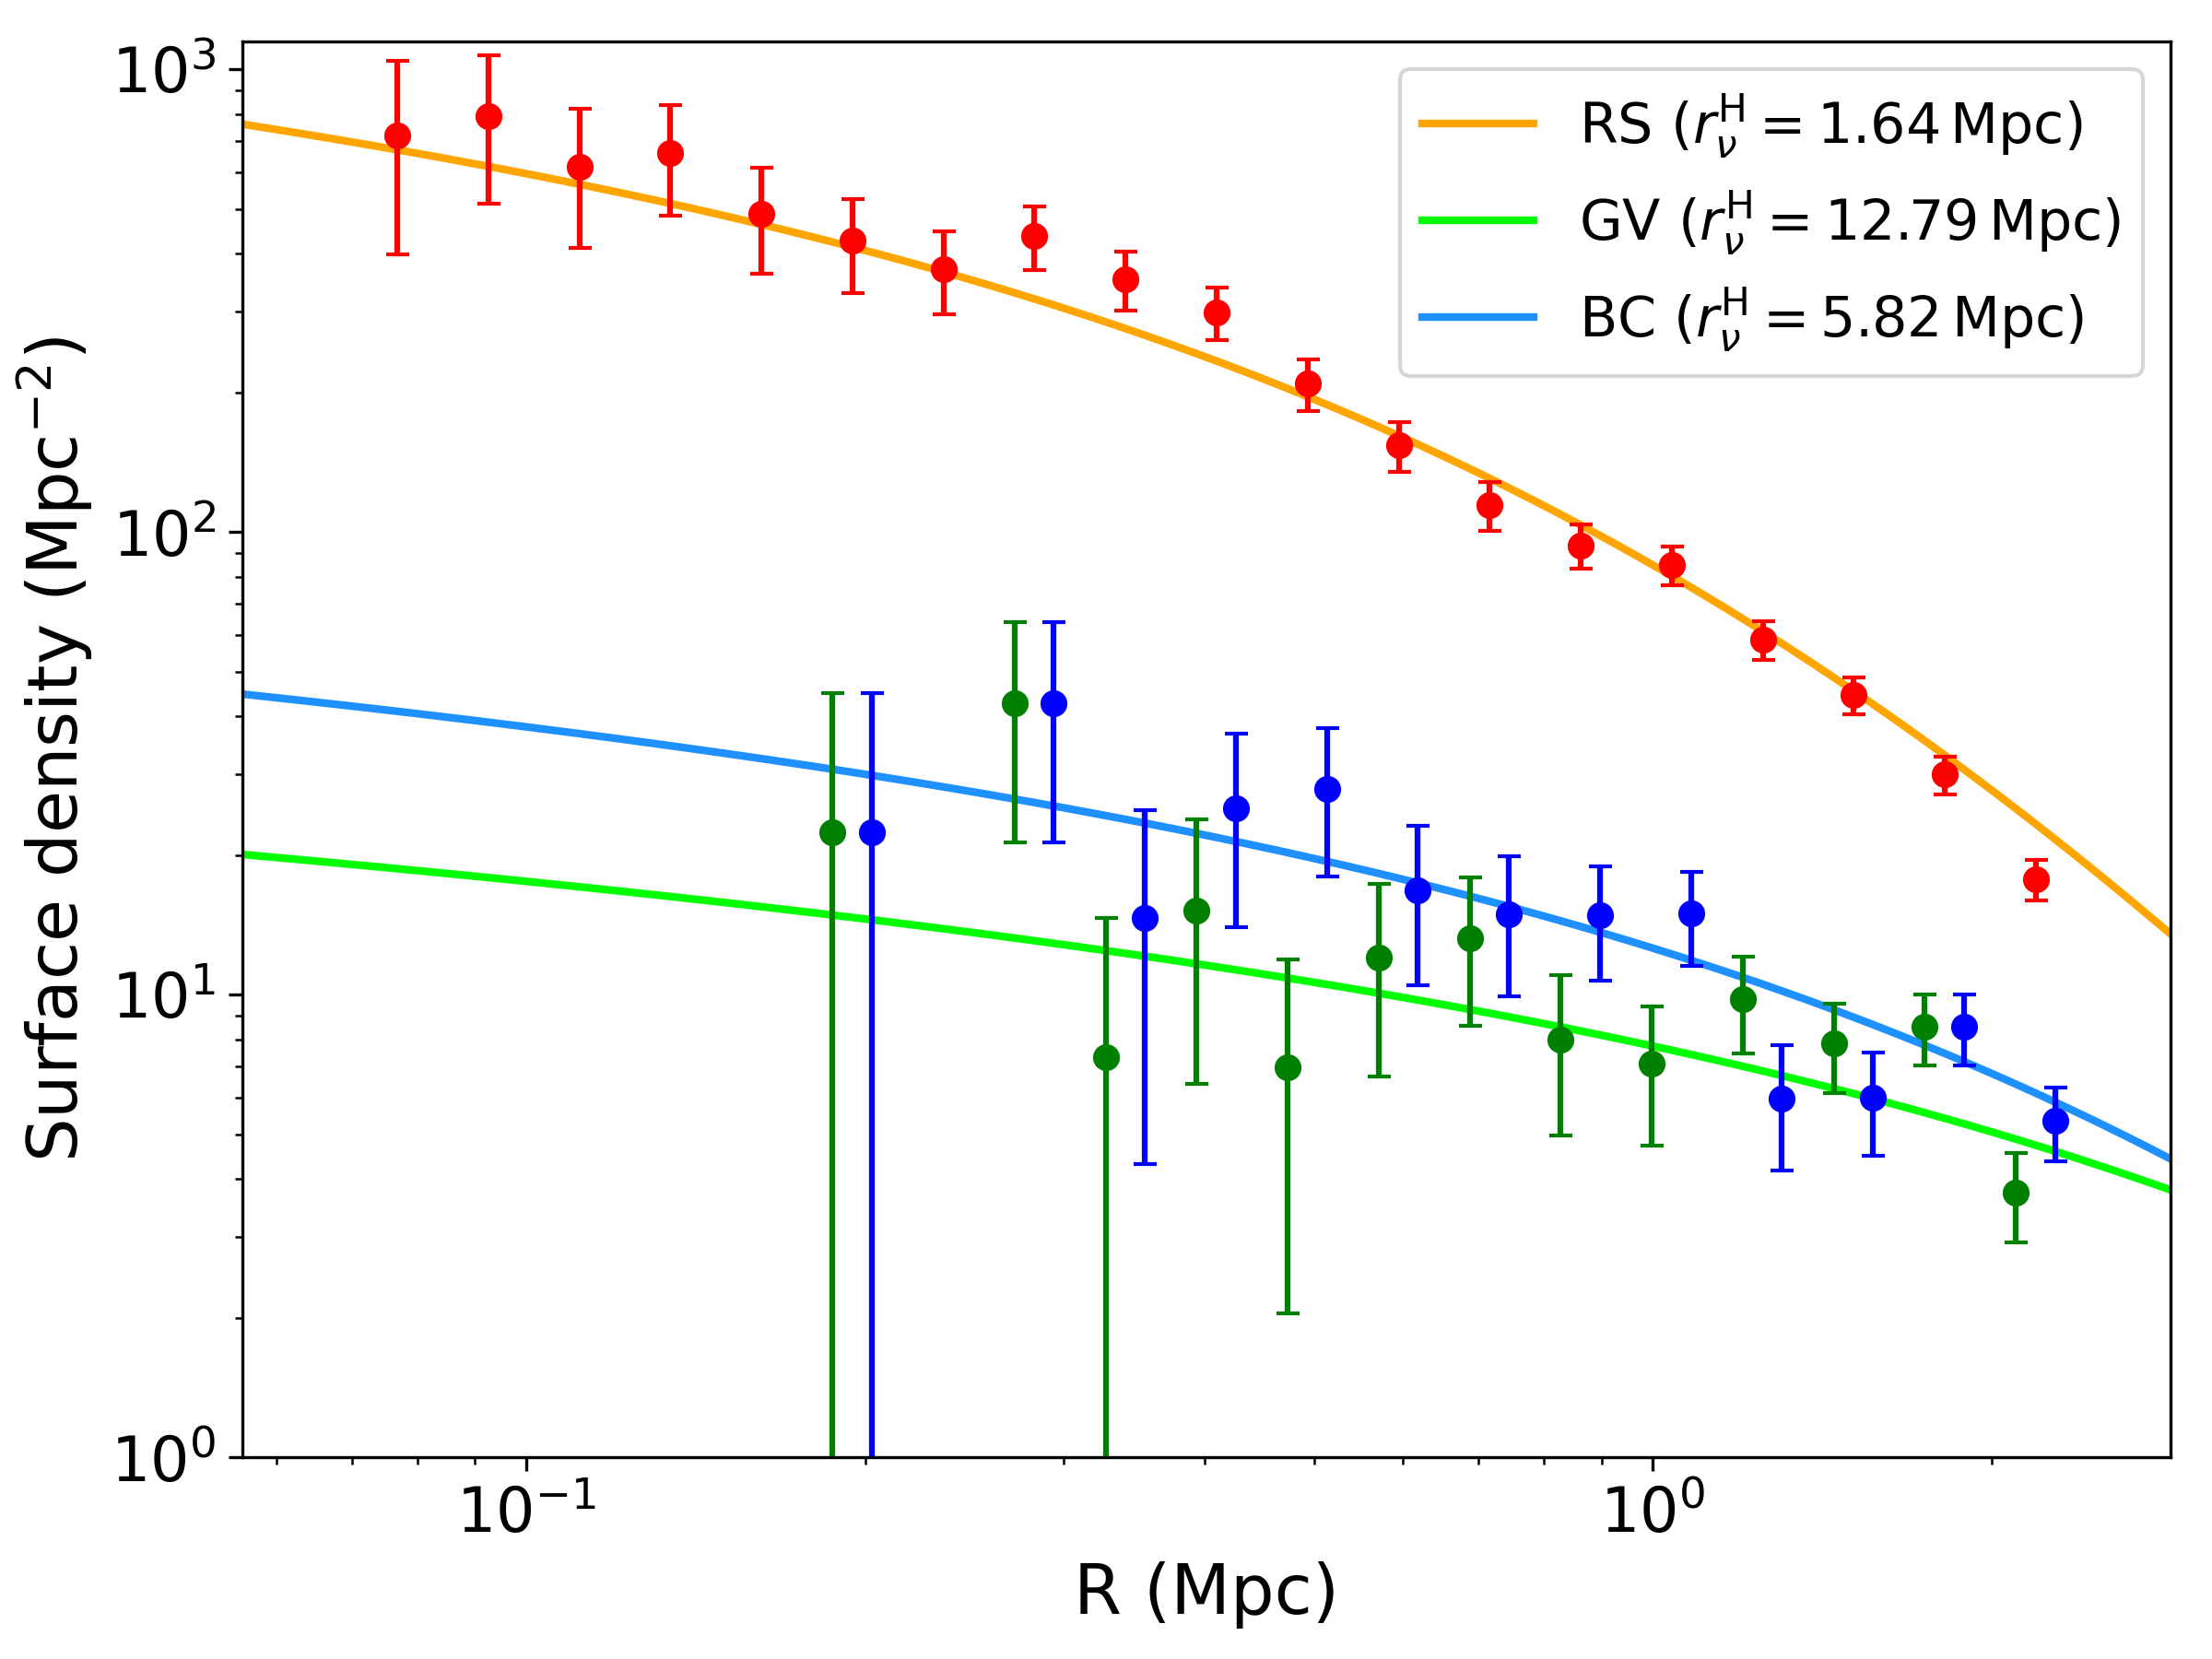
\includegraphics[width=0.9\linewidth]{images/surface_density_3pop_Her_superposed.png}
    \caption{Surface density profiles of RS (red), GV (green), and BC (blue) galaxies in the Coma Cluster fitted with projected Hernquist models with, respectively, $r_\nu^{\rm H} = 1.64\, \text{Mpc}, 12.79 \,\text{Mpc} \,\text{and}\, 5.82 \, \text{Mpc}$. The error bars correspond to the Poisson uncertainties.}
    \label{fig:surface_density_subsamples}
\end{figure} 


\section{Multi-component mass profile} \label{app:mc}
In Fig.~\ref{fig:multicompoent} we plot the total mass profile of Coma obtained by using the sample of galaxies with no distinction in the three colour classes, in the projected radial range $R \in [0.10, 2.3]$ Mpc and assuming the multi-component mass model of eq.~\eqref{eq:multic}. The grey bands and the black solid line indicate the radial profile of the diffuse DM component, parametrised as a gNFW. While the virial radius (and so the dark matter mass) is well constrained, $r_{200}^{\rm DM} = 1.94^{+0.09}_{-0.06}$ Mpc, the scale radius $r_{\rm s}$ and the slope $\alpha$ are completely degenerate. This is not surprising; as shown in \textit{e.g.}~\cite{Sartoris_2020} and \cite{Biviano:2023oyf}, to break this degeneracy using kinematic analyses requires spectroscopic data of the stellar velocity dispersion in the BCG to be included in the fit.

\begin{figure}[!h]
    \centering
    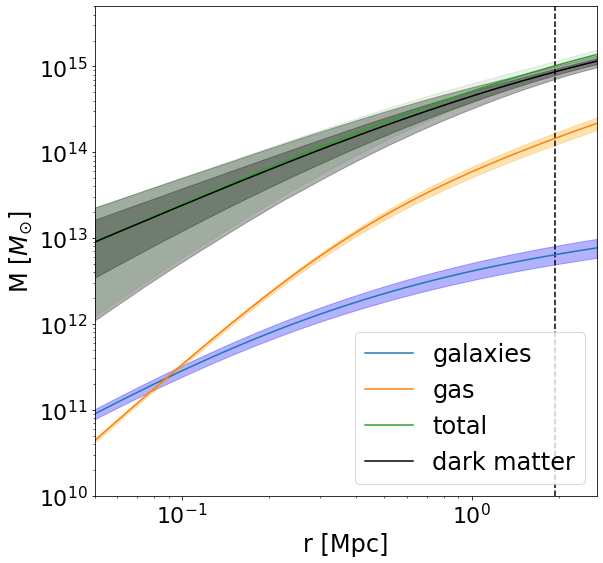
\includegraphics[width=0.9\linewidth]{images/multicomponent_gNFW.png}
    \caption{Total mass profile (green solid line) of Coma with its 95\% confidence interval (green shaded region), along with the mass of the different components: galaxies (blue),  gas (orange),  DM (black). The grey inner and outer shaded regions indicate the 68\% and 95\% confidence region of the DM profile, respectively. The black dashed vertical line corresponds to $r_{200}^{\rm DM} = 1.94^{+0.09}_{-0.06}$ Mpc. The orange and blue bands represent the 68\% limits of the gas and galaxies mass profiles.}
    \label{fig:multicompoent}
\end{figure} 


\section{Mass and orbital anisotropy study for low- and high-mass galaxies}
\label{app:high-vs-low-mass}

As mentioned in Sect. \ref{subsec:diff_sample_mamposst}, we split the full sample in two equal population (662 members) stellar mass bins, with the threshold at $\log (M_*/M_\odot) = 9.1$, to check differences in the estimated mass and anisotropy parameters. RS galaxies are the most evenly distributed between the two bins, with 45.8\% below the mass threshold and 54.2\% above it. GV galaxies show a similarly balanced distribution, with 55.4\% with low mass and 44.6\% with high mass. In contrast, BC galaxies are strongly skewed towards the low-mass regime, where 75.3\% of them are found. The colour composition of the two stellar mass bins can be found in Table \ref{tab:composition_colors}. 

\begin{table}
\centering
\renewcommand{\arraystretch}{1.3} % <-- più spazio tra righe
\caption{Fraction of RS, GV and BC galaxies in the two stellar-mass bins.}
\begin{tabular}{lcc}
\hline
Population & $\log (M_\star/M_\odot) < 9.1$ & $\log (M_\star/M_\odot) > 9.1$ \\
\hline
RS & 71.6\% & 85.3\% \\
GV & 10.9\% & 8.9\% \\
BC & 17.5\% & 5.8\% \\
\hline
\label{tab:composition_colors}
\end{tabular}
\end{table}

Following the same strategy adopted for the colour classes, we first ran \textsc{MG-MAMPOSSt} with flat priors (same as Table \ref{tab:priors_flat}) to independently estimate the mass parameters and then we employed Gaussian priors on the mass from the joint analysis of Sect. \ref{full_sample_mamposst} to compare the anisotropy profiles. The best fit parameters are reported in Table \ref{tab:massbins_results} and Table \ref{tab:massbins_results_withpriors}. Note that we have repeated the numerical density profile fit for these new subclasses (as in Sect. \ref{num_density_methods}), to ensure that Gaussian priors on $r_\nu^{\rm H}$ are appropriate, finding the best fit values of $r_\nu^{\rm H}=1.70_{-0.61}^{+0.03} \, \mathrm{Mpc}$ for the low-mass and $r_\nu^{\rm H}=1.98_{-0.11}^{+0.41} \, \mathrm{Mpc}$ for the high-mass galaxies.

\begin{table}
\centering
\caption{Best fit parameters for low-mass and high-mass galaxies.}
\renewcommand{\arraystretch}{1.3}
\begin{tabular}{lccc}
\hline
{Parameter} & {Low-mass} & {High-mass}  \\
\hline
       
       $r_{200} \, (\mathrm{Mpc})$ & $2.23_{-0.12}^{+0.10}$ & $2.13_{-0.09}^{+0.06}$  \\
       $r_{\rm s} \, (\mathrm{Mpc})$ & $0.82_{-0.52}^{+0.55}$ & $0.58_{-0.35}^{+0.10}$ \\
       $r_\nu^{\rm H} \, (\mathrm{Mpc})$ & $2.09_{-0.28}^{+0.22}$ & $1.35_{-0.10}^{+0.20}$  \\
       $\mathcal{A}_0$ & 
       $1.42_{-0.51}^{+0.63}$ & $1.14_{-0.42}^{+0.92}$  \\
       $\mathcal{A}_\infty$ & $1.20_{-0.32}^{+0.25}$ & $1.42_{-0.47}^{+0.14}$  \\
          
\hline
\end{tabular}
\caption*{\footnotesize \textbf{Notes.} The employed mass and anisotropy models are NFW and gOM, respectively. The assumed priors, for these runs, are broad and flat, except for $r_\nu^{\rm H}$, for which we considered informative priors based on the best fit values for each subsample.}
\label{tab:massbins_results}
\end{table}


As expected, the mass parameters ($r_{\rm s}$ and $r_{200}$) estimated from the low-mass sample are higher than those obtained from the high-mass one, given the contribute of the vast majority of BC galaxies. Both the anisotropy profiles (Fig.~\ref{fig:anis_massbins}) show a predominant radial component, with the high-mass galaxies showing an even more radial behaviour.




\begin{table}
\centering
\caption{Same as Table \ref{tab:massbins_results}, but for the runs with Gaussian priors on $r_{200}$ and $r_{\rm{s}}$ from the joint analysis of Sect. \ref{full_sample_mamposst}.}
\renewcommand{\arraystretch}{1.3}
\begin{tabular}{lccc}
\hline
{Parameter} & {Low-mass} & {High-mass} \\
\hline
       
       $r_{200} \, (\mathrm{Mpc})$ & $2.18_{-0.05}^{+0.04}$ & $2.13_{-0.06}^{+0.03}$  \\
       $r_{\rm s} \, (\mathrm{Mpc})$ & $0.69_{-0.32}^{+0.03}$ & $0.57_{-0.26}^{+0.04}$  \\
       $r_\nu^{\rm H} \, (\mathrm{Mpc})$ & $1.91_{-0.11}^{+0.18}$ & $1.44_{-0.09}^{+0.16}$  \\
       $\mathcal{A}_0$ & 
       $1.12_{-0.47}^{+0.61}$ & $1.25_{-0.54}^{+0.97}$  \\
       $\mathcal{A}_\infty$ & $1.23_{-0.29}^{+0.13}$ & $1.27_{-0.27}^{+0.17}$  \\
          
\hline
\end{tabular}
\caption*{\footnotesize \textbf{Notes.} Gaussian priors on $r_\nu^{\rm H}$ are based on the estimates of Sect. \ref{num_density_methods}, while those for $\mathcal{A}_0$ and $\mathcal{A}_\infty$ are flat (same as Table \ref{tab:priors_flat}).}
\label{tab:massbins_results_withpriors}
\end{table}

\begin{figure*}
    \centering
    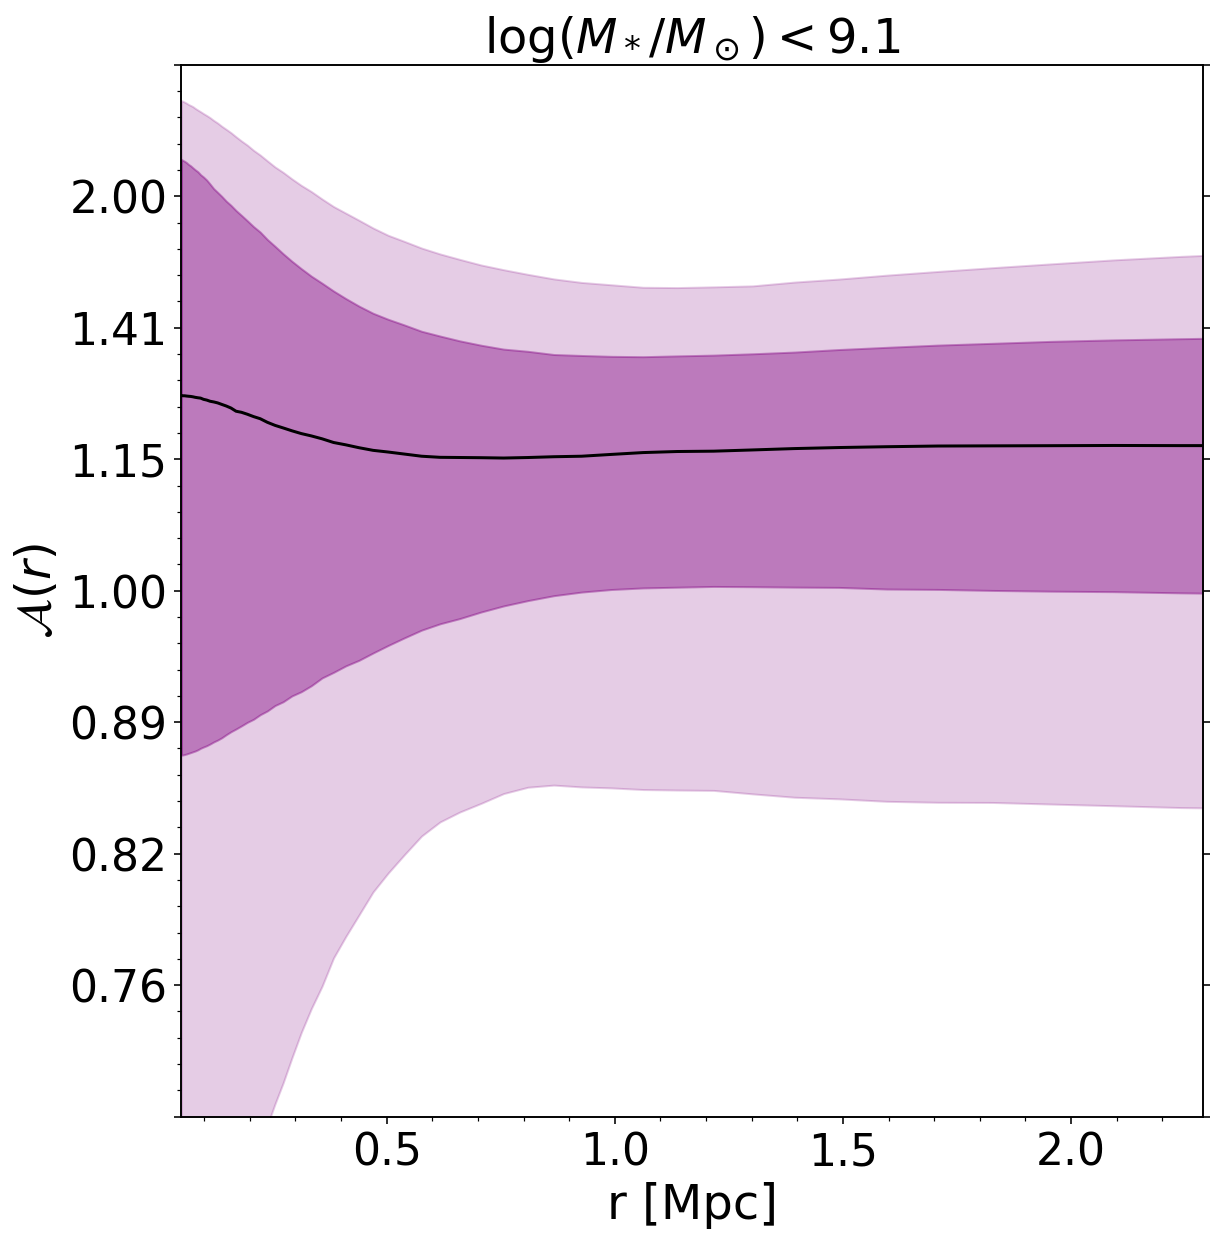
\includegraphics[width=0.35\linewidth]{images/low_mass.png}
    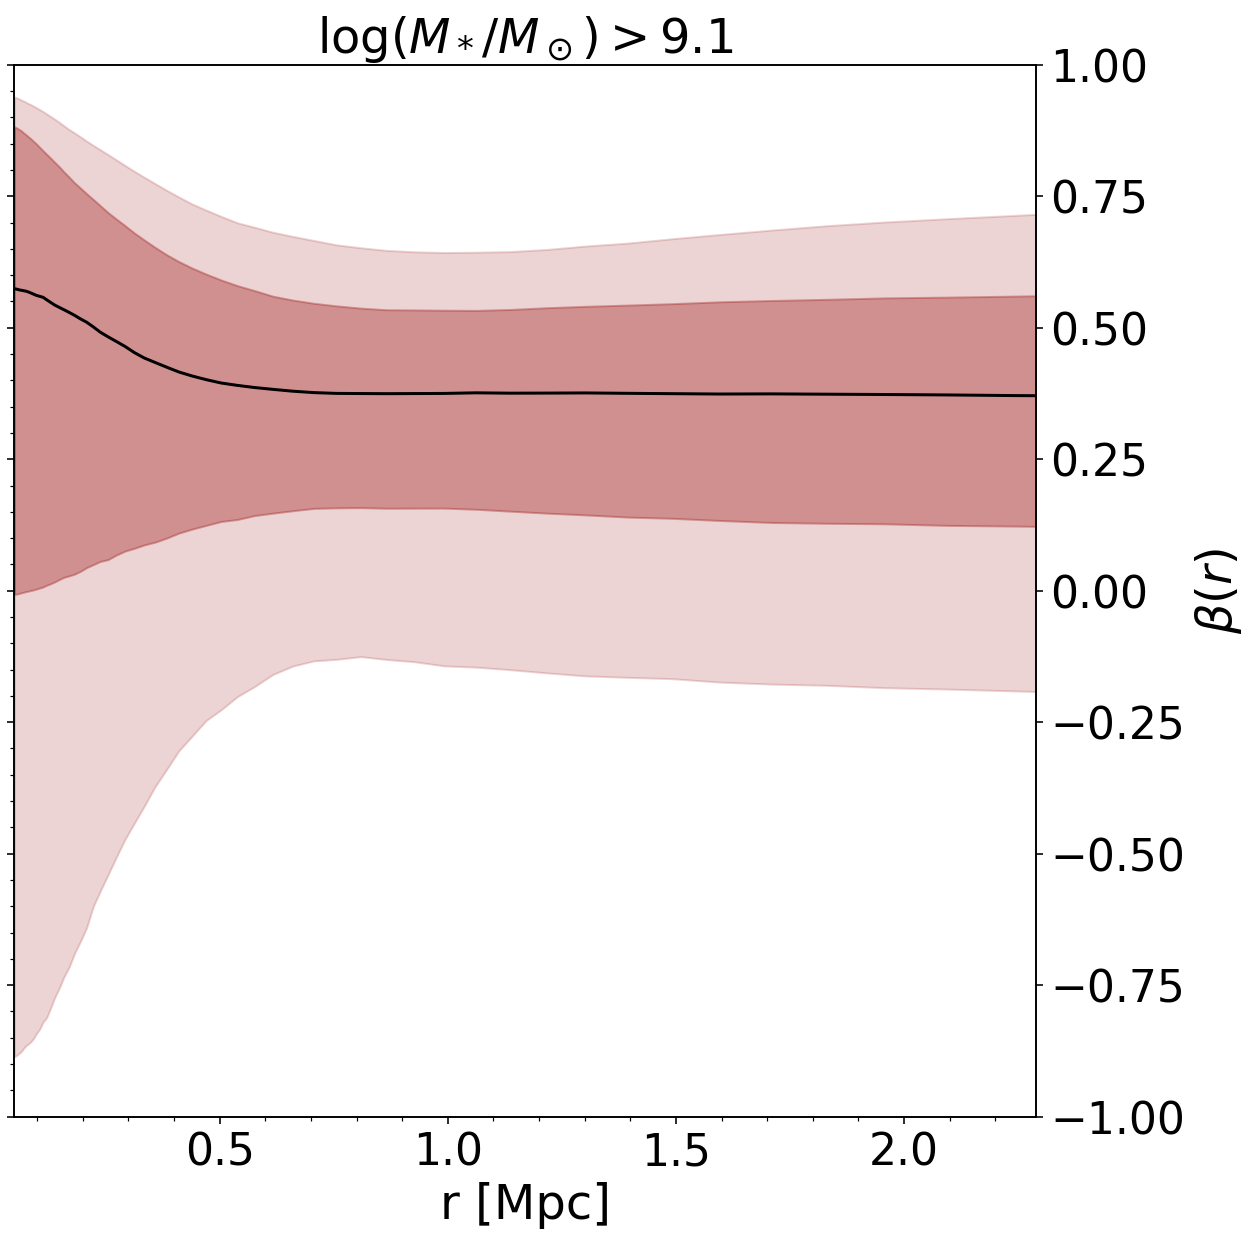
\includegraphics[width=0.3615\linewidth]{images/high_mass.png}

    \caption{Estimated anisotropy profiles in NFW gOM runs with Gaussian priors on the mass (coming from the joint results of Sect. \ref{full_sample_mamposst}) for low-mass (left) and high-mass (right) galaxies, separately. The coloured and shaded regions indicate 1$\,\sigma$ and 2$\,\sigma$ confidence intervals, respectively. Solid curves are the median profiles of each MCMC chain.}
    \label{fig:anis_massbins}
\end{figure*} 





%%%%%%%%%%%%%%%%%%%% REFERENCES %%%%%%%%%%%%%%%%%%

% The best way to enter references is to use BibTeX:

 % if your bibtex file is called example.bib

\end{document}


